\documentclass[bacharelado]{unb-cic}
\usepackage[american,brazil]{babel}
\usepackage[T1]{fontenc}
\usepackage{indentfirst}
\usepackage{natbib}
\usepackage{xcolor,graphicx,url}
\usepackage[utf8]{inputenc}
\usepackage{listings}
\usepackage{color}

\definecolor{dkgreen}{rgb}{0,0.6,0}
\definecolor{gray}{rgb}{0.5,0.5,0.5}
\definecolor{mauve}{rgb}{0.58,0,0.82}

\lstset{frame=tb,
	language=sh,
	aboveskip=3mm,
	belowskip=3mm,
	showstringspaces=false,
	columns=flexible,
	basicstyle={\small\ttfamily},
	numbers=none,
	numberstyle=\tiny\color{gray},
	keywordstyle=\color{blue},
	commentstyle=\color{dkgreen},
	stringstyle=\color{mauve},
	breaklines=true,
	breakatwhitespace=true,
	tabsize=3
}

%\bibpunct[; ]{(}{)}{,}{a}{}{;}%muda colchetes para parênteses

% definições prévias do documento
\title{Aplicação de RAID em Sistema de Arquivos Distribuídos}

\orientador{\prof \dr Eduardo A. P. Alchieri}{CIC/UnB}

\coordenador{\prof \dr Rodrigo Bonifacio de Almeida}{CIC/UnB}

\diamesano{18}{Junho}{2016}

                           
\membrobanca{\prof\dr Professor I}{CIC/UnB}

\membrobanca{\prof \dr Professor II}{CIC/UnB}

\autor{Diogo Assis}{Ferreira} 
\coautor {Getúlio Yassuyuki}{Matayoshi}


\CDU{004.4}

\palavraschave{RAID, BFT SMaRt, Sistema de arquivo distribuído}
\keywords{RAID, BFT SMaRt, Distribuited file sistem}


\begin{document}

\maketitle

\pretextual

\begin{agradecimentos}
Foi uma tarefa árdua chegar ao momento atual, monografia completa, créditos conquistados, colação marcada. Digo que a missão foi complicada pois exigiu dezenas de horas de estudo, noites em claro, programas que não compilavam, \textit{segmentation fault} aparentemente sem explicação, cálculos que não batiam, diversos finais de semana na faculdade. Porém nenhuma dessas frustrações supera a satisfação de conseguir superar tais problemas, a conta realizada com precisão, o programa otimizado que executa com exatidão, a prova com sabor de vitória, tudo levando àquela bela e merecida noite de sono antes do ciclo recomeçar. Por isso digo que não foi fácil, mas foi enriquecedor, o quanto aprendi, o quanto vivenciei, são experiências preciosas que carregarei com carinho e orgulho. Entretanto, devo ressaltar que essa trajetória não foi percorrida por mim sozinho, em todo o momento eu recebia direta ou indiretamente o apoio de pessoas importantes. Meu pai, sempre disposto a preparar uma bela refeição entre meus estudos, minha mãe, preocupada todas as vezes em que ficava até tarde na UnB, minha irmã, sempre pronta pra me pentelhar (e ajudar a aliviar todo o estresse dos estudos), Talita, minha namorada, sempre disposta a me receber com carinho e confortar todas minhas (várias) lamurias, minha família: avôs, tias, primos também dando seu suporte da forma que podiam, amigos e colegas que passavam os momentos de desespero e diversão na faculdade ou fora dela, sou muito grato a todos. Contudo, gostaria de expressar minha gratidão em especifico à meu orientador que teve muita paciência, boa vontade e bom humor para me ajudar nessa tortuosa parte final do curso e a meu parceiro, Getúlio, que foi de fundamental importância para a conclusão deste trabalho, obrigado! Obrigado a todos! E até o próximo desafio!
\\

Diogo Assis Ferreira
\\

\end{agradecimentos}

\begin{resumo}
Este trabalho tem como foco a construção de um sistema de arquivos distribuídos que é tolerante a falhas, sem prejuízo de desempenho e que consuma menor quantidade de \textit{overhead} do que o sistema apresentado pelo método de replicação de dados tradicional. A fim de alcançar tal objetivo foram utilizadas as características inerentes ao conceito do RAID 0, RAID 1 e RAID 5, as quais possibilitaram o teste das latências e o teste do \textit{throughput} das operações de leitura e escrita com arquivos de quatro tamanhos distintos, sendo esses 1KB, 100KB, 1MB e 10MB. A coleta e a análise dos dados resultou na conclusão de que o sistema alcança o objetivo proposto, sendo que, quando executado sob as parametrizações do RAID 5, o desempenho geral é superior se comparado aos outros dois modelos de RAID implementados.
\\

\end{resumo}

\selectlanguage{american}

\begin{abstract}
This work has as its focus the construction of a fault tolerant distributed file system, without compromising performance, that consumes a lesser quantity of overhead than the system presented by the traditional data replication method. In order to achieve this goal, inherent characteristics of the concept of the RAID 0, RAID 1 and RAID 5 were used, which enabled the test of the latencies and the test of the throughput of the reading and writing operations with four distinct file sizes, these being 1KB, 100KB, 1MB and 10MB. The gathering and the analysis of these data resulted in the conclusion that the system reaches the proposed objective, being that, when run under the parameterizations of the RAID 5, the overall perfomance is superior if compared to the other two implemented RAID models.
\\

\end{abstract}

\selectlanguage{brazil}
\tableofcontents
\listoffigures
\listoftables

\textual

\chapter{Introdução}

 

	



	\section{Contextualização}
	Atualmente, o volumes de dados que são processados e armazenados no mundo inteiro está crescendo cada vez mais, impulsionado intensamente com o aumento da capacidade de processamento e armazenamento de dados e a popularização da internet entre as pessoas. Na área da ciência surgiu um novo e quarto paradigma científico, seguindo de ciência empírica, ciência lógica e ciência computacional, chamado de \textit{data-intensive science}~\cite{hey2009}, proposto pelo cientista da computação pioneiro Jim Gray. Esse paradigma é caracterizado por focalizar na intensiva coleta e acúmulo de dados, para serem submetidos em análise a fim de extrair as informações vantajosas. Várias empresas e organizações estão dando atenção especial em \textit{big data}, um novo conceito que surgiu com aplicação do paradigma \textit{data-intensive science}, cujo consiste em conjunto de dados não estruturados extremamente amplo, e por esse motivo, é impossível de ser processado por um computador convencional. O \textit{big data} é usado para analisar as relações complexas que existem entre enorme quantidade de dados contidos nele para obter as informações como previsões ou tendencias, onde geralmente são impossíveis de serem obtidas se fosse usado um volume convencional de dados. Esse crescimento de volume de dados não afetou somente áreas de negócio ou cientifico, mas também os usuários finais, com foco em armazenamento de dados, evidenciado com aumento de capacidade do disco rígido contido em um computador pessoal ou aumento de demanda por um serviço de armazenamento remoto baseando em conceitos de computação em nuvem, chamado de \textit{cloud storage service}.
	\\ 

	%Atualmente, a importância de coleta e acúmulo de dados para submeter em análise a fim de extrair as informações vantajosas está sendo discutida em diversas áreas. Este fato é evidenciado com o surgimento de , e definição de novo conceito denominado de \textit{big data}, o conjunto de dados extremamente amplo, e por esse motivo, é impossível de ser processado por um computador convencional. \\
	
	Para ter noção concreta de tamanho de dados processados, apresentamos como exemplo alguns casos da utilização de \textit{big data}. O CERN, o maior laboratório de física de partículas do mundo, que tinha anunciado em 2013 que registrou mais de 100 petabytes de dados de pesquisa ao longo dos últimos 20 anos, em que 75 petabytes destes dados foram gerado com as experiências de colisão no \textit{Large Hadron Collider} (LHC), nos últimos 3 anos~\cite{cern}. Também temos o Facebook, um serviço de rede social que em 2012 foi considerado maior do mundo, possui um \textit{data warehouse} que armazena mais de 300 petabytes de dados acumulados, e ainda 600 terabytes de dados chegam a cada dia~\cite{facebook14}. No caso de Dropbox, o serviço \textit{cloud storage} mais pupular do mundo, oferece 2 gigabytes de espaço básico para todos os usuários, podendo ser aumentado até espaço ilimitado dependendo de plano, e registrou mais de 300.000.000 usuários cadastrados~\cite{dropbox}, implicando que é necessário manter o espaço de armazenamento no mínimo 600 petabytes disponível a qualquer instante para suprir todos seus usuários.\\
	
	Como mostra em exemplos apresentados, um volume imenso de dados estão sendo intensamente coletado e submetido a análise. No caso do Dropbox que possui um sistema com 600 petabytes de capacidade de armazenamento estimada, implicando que será necessário, quando for usado um disco rígido com 2 terabytes de capacidade na sua composição, utilizar 300.000 dispositivos, sendo extremamente difícil de ser equipados em uma máquina que pode ser encontrada normalmente. Existe também problema com gerenciamento de dados, pois nenhum computador convencional possui o desempenho suficiente para tratamento de dados nesta escala. \\
	
	
	Uma solução tipicamente adotada  para  resolver esta questão de armazenar os dados de grande porte é aumentar igualmente a escala do sistema de armazenamento, introduzindo um sistema de arquivo distribuído.
	Esta abordagem é mais escolhido que as outras pelo fato de que apresenta uma vantagem em relação ao incremento da escala do sistema, em que neste processo o sistema distribuído possui mais facilidade e o menor custo relativo comparados com outras abordagens. 
	Consiste de um conjunto de vários computadores, chamados de nós, fisicamente distribuídos e conectados através de uma rede. 
	O nó que constitui o sistema pode ser um computador comum ou até um de grande porte, como servidor, e quando precisa aumentar o desempenho do sistema todo basta adicionar novos nós no conjunto. 
	Contudo, na abordagem de armazenamento distribuído quase sempre é  acompanhado com questão de degradação da confiabilidade de conteúdos armazenados. 
	Como os dados que estão contidos no sistema estão localizados distribuidamente sobre vários nós, o risco da perda ou alteração de algum destes dados cresce cada vez que aumenta a escala do sistema, pois a probabilidade de ocorrer uma falha em algum dos componentes cresce proporcionalmente com aumento da quantidade de dispositivos envolvidos.
	Para solucionar esse problema de confiabilidade dos conteúdos armazenados, muitos sistemas de arquivos distribuídos introduzem alguns mecanismos para tolerar possíveis falhas. 
	Um deles é a atribuição da redundância nos arquivos, em que são realizados principalmente com simples criação das cópias de segurança, chamadas de réplicas, para cada um dos arquivos encontrados no sistema. 
	\\
	
	A atribuição de redundância consegue impedir o decaimento da confiabilidade dos arquivos, mas isto tem um custo extra.
	Se um arquivo é protegido com duas réplicas significa que no sistema existem três dados idênticos, consumindo o triplo de espaço que este arquivo realmente ocupa no dispositivo de armazenamento. 
	Assim, manter a grande quantidade de dados sem degradar a segurança está tornando-se cada vez mais custoso com aumento de volume dos dados armazenados, mesmo utilizando uma solução mais adequada possível. 
	A situação agrava ainda mais quando a ordem de tamanho chega em centenas de petabytes, como ocorre no caso de um conjunto de dados considerado como \textit{big data} ou no caso de arquivos gravados por todos os usuários de algum serviço de armazenamento nas nuvens. 
	%Para lidar com essa complexidade, uma opção é o uso da abordagem de \textit{State Machine Replication} (SMR), ou a replicação de máquina de estado, que possui o objetivo de aumentar o desempenho e a capacidade de sistema ou de prover tolerância a falha~\cite{alchieri}, criando as réplicas de computador ou servidor.\\
	
	%O uso do sistema de arquivos distribuídos resolve a questão de capacidade para armazenamento de dados de grande porte com incremento de escala, acrescentando um servidor quando for necessário. Este método é bem eficiente, prático e relativamente barato, contudo pode se tornar custoso, pois não ocorre somente adicionamento das máquinas, mas também a substituição, seja parcial ou inteira, dos componentes que apresentou algum defeito, e certamente isso ocorre com uma frequência significante e ser intenso cada vez que aumenta a escala, acumulando o custo ao longo do tempo.\\
	

	
	
	
	

 

	



\section{Objetivo}

A taxa de espaço extra necessário para armazenar um arquivo, representada pela parte redundante, é chamado de \textit{overhead} de espaço.
Por exemplo, na replicação de arquivo que possui apenas uma réplica, o \textit{overhead} é de 100\%, pois para cada um arquivo será criada uma parte redundante.
O nosso objetivo neste trabalho é a construção de um sistema de arquivos distribuídos tolerante a falhas de forma que apresenta menor \textit{overhead} de espaço que o método da replicação de arquivo tradicional, e ao mesmo tempo apresente um bom desempenho.
\\

Para isso, nós observamos conceitos da tecnologia RAID, pois notamos alguns pontos semelhantes com o sistema de arquivos distribuídos, como o armazenamento de forma distribuído e a preocupação com a segurança dos arquivos.
Além disso, a utilização da replicação de arquivo e de outro método para atribuição da redundância também foi motivo para colocar atenção nesta tecnologia.
A outra forma de criar as partes redundantes é a geração de paridades, que são calculadas baseando-se em blocos divididos a partir do próprio arquivo.
Dessa forma, é possível reduzir o \textit{overhead} de espaço até 50\%, a metade da replicação com uma cópia, quando as paridades forem geradas de forma mais simples, ou até menos, dependendo da condição utilizada para calcular a paridade.
\\

Também notamos o fato de que a tecnologia RAID foi inicialmente desenvolvida para aumentar a taxa de transferência da unidade de armazenamento.
A motivação inicial desta invenção era reusar os discos rígidos que não estavam mais em uso, por serem substituídos por outros mais novos com melhor performance.
O problema para fazer o reuso dos dispositivos era a baixa velocidade de leitura/escrita que estes apresentavam, por serem aparelhos relativamente velhos. 
Para cobrir esta baixa velocidade de transferência, os discos foram colocados para trabalhar em conjunto, ou seja, fazer um acesso simultâneo em vários discos para aumentar a vazão total de dados transferidos, resultando em aumento da taxa de transferência .
Assim, a introdução de conceito do RAID, não trata apenas de questão da segurança de arquivos, mas também no desempenho do sistema.  
\\
%Como uma consequência extra de introdução do RAID, é esperado que tenha a melhoria na distribuição da carga de operações entre os servidores, pois os arquivos estão armazenados espalhadamente sobre todos os nós do sistema, levando na redução da probabilidade de ocorrer a concentração de acesso em um dos nós.

Para que o armazenamento de arquivo seja administrado de forma eficiente, contribuindo para aumento do desempenho do sistema, adotamos uma abordagem que separa o arquivo em duas partes para distribuir a carga de gerenciamento. 
Uma parte são os metadados, que guardam as informações do arquivo, como nome, tamanho ou localização. E a outra parte é o dado, que armazena o próprio conteúdo deste arquivo. 
Desta forma, o sistema será constituído por dois tipos diferentes de conjunto dos servidores, um que administra os metadados dos arquivos e outro que armazena os dados dos arquivos. 
\\

Da mesma forma que a confiabilidade do conteúdo dos arquivos é assegurado por conceito de RAID, os metadados armazenados também precisam ser protegidos.
Porém, não podemos usar o RAID para fazer isso, pois nos servidores de metadados não acontecem simples entrada/saída de dados, mas também fornecem um serviço para indicar localização de conteúdo dos arquivos. 
Por isso, para garantir a segurança dos metadados, junto com o serviço, utilizamos o \textit{BFT-SMaRt}, uma biblioteca em Java que disponibiliza as ferramentas para desenvolver um serviço tolerante a falhas, baseado na técnica de replicação de serviço.
\\


%e da mesma forma os metadados serão protegidos através de BFT-SMaRt, uma biblioteca JAVA que fornece a tolerância a falha no serviço, realizada com uso de método de replicação do serviço.\\


Assim, o nosso trabalho está focalizado em construção de um sistema de arquivos distribuídos utilizando os conceitos de RAID.
Será implementado algumas configurações de RAID, incluindo uma que utiliza a replicação de arquivo e outra que utiliza a geração de paridade, e posteriormente será feito a comparação entre as configurações desenvolvidas no sistema, para verificar a diferença de desempenho entre elas.
\\

%Também será feito a comparação de desempenho entre os dois sistemas, um que usa método de replicação e outro que usa método de RAID.
%Comparando os dois métodos de redundância, será possível a visualização das vantagens e desvantagens que existem entre eles.












	\section{Organização de capítulos}
	
	Os capítulos estão organizados de seguinte forma. 
	O Capítulo 2 apresenta os conceitos sobre sistema de arquivos distribuído, explicando as principais características que esse tipo de sistema apresenta.  
	O Capítulo 3 apresenta os princípios do \textit{BTF-SMaRt}, uma biblioteca que realiza a replicação de serviços para prover a tolerância a falhas no sistema, assim como os protocolos centrais e sua implementação.
	O Capítulo 4 apresenta os conceitos da tecnologia RAID.
	O Capítulo 5 descreve o desenvolvimento do sistema proposto.
	O Capítulo 6 explica como os experimentos foram realizados além de analisar os resultados obtidos.
	Por fim, o sétimo capítulo apresenta a conclusão deste trabalho, além dos trabalhos para futuro.
%\chapter{Fundamentação}
\chapter{Sistema de arquivos distribuído}


 

	


Este capítulo introduz o que é um sistema de arquivos distribuído. De modo didático, primeiro é explanado o que é um sistema distribuído, o que são metadados, e então, é apresentado a definição e características de um sistema de arquivos distribuído.


	%\section{Sistema de arquivos distribuído}
	
	\section{Sistema distribuído}
	Hoje em dia, podem ser encontrada diversas tarefas computacionais que são impossíveis de ser processadas por um computador comum, devido a simples limitação da capacidade de processamento que uma máquina pode atingir. A solução tipicamente tomada por muitas organizações é o uso de sistema distribuído, no qual possui algumas vantagens comparado a um sistema centralizado, como pode ser visto a seguir.
	
	\begin{itemize}
		\item Melhor relação custo-benefício;
		\item Capacidade de processamento além dos limites práticos de sistema centralizado;
		\item Alta confiabilidade e disponibilidade;
		\item Relação linear entre crescimento de custo e desempenho.
	\end{itemize}
	Os sistemas de computação distribuída são caracterizados pela sua estrutura, cuja consiste em interação entre um grande número de dispositivos que executam seus próprios programas, mas que são afetados recebendo as mensagens ou observando a memória compartilhada de outros dispositivos.
	\\
	
	Existem várias definições e pontos de vista sobre o que são sistemas distribuídos. Coulouris~\cite{coulouris06} define um sistema distribuído como "um sistema no qual os componentes de hardware e software localizadas nos computadores conectados por rede comunicam e coordenam suas ações somente por passagem de mensagens", e Tanenbaum~\cite{tanenbaum07} define como "uma coleção de computadores independentes que aparenta ao usuário ser um computador único". Leslie Lamport, um famoso pesquisador sobre sistema distribuído, disse uma vez que "um sistema distribuído é aquele em que é impedido de prosseguir com seu trabalho devido a uma falha de algum computador que nunca ouviu falar" refletindo o grande número de desafios enfrentados pelos projetistas de sistemas distribuídos.
	\\
	
	Assim, quando um sistema distribuído aumenta o seu tamanho, torna-se cada vez mais difícil de prever ou mesmo entender o seu comportamento. A parte da razão para isso é simples falta de ferramentas que gerenciam a complexidade e outra parte é que um sistema distribuído de grande porte traz consigo a quantidade enorme de não-determinismo inerente, os eventos imprevisíveis, como atrasos nas chegadas de mensagem, súbito falhas de componentes, ou em caso extremo, as ações nefastas de defeitos ou máquinas maliciosos que agem opostamente para os objetivos do sistema como um todo.
	
		\section{Metadados} 
		
		Os sistemas de arquivos, como ambientes propícios para a recuperação de informações, têm na utilização de metadados a padronização das formas de representação e a possibilidade de garantia de interoperabilidade entre sistemas, favorecendo a integridade e a acessibilidade dos recursos informacionais de forma eficiente pelo usuário final. Os metadados são "dodos de dodos", ou seja, as informações essenciais sobre os arquivos armazenados, indispensáveis para fazer o gerenciamento de arquivos, indicando as características inerentes deles. A Tabela~\ref{tab:metadado} mostra os atributos encontrados em um metadado.
		
		\capstartfalse
		\begin{table} [htb]
			\caption{Elementos de metadados}
			\centering
			\begin{tabular}{|l|l|} \hline
				\textbf{Informação} & \textbf{Descrição} \\ \hline
				
				Nome do arquivo		& O nome do arquivo, incluindo o caminho do diretório.\\ \hline
				Proprietário		& O identificador de usuário que é o dono do arquivo.\\ \hline
				Data de criação     & Data que o arquivo foi criado.\\ \hline
				Data de acesso		& Data de último acesso do arquivo. \\ \hline
				Data de atualização	& Data de última atualização feito sobre o arquivo. \\ \hline
				Tamanho				& Espaço ocupado pelo arquivo ao longo do disco. \\ \hline
				Tipo de arquivo		& indica se ele é uma pasta ou um arquivo normal.  \\ \hline
				Modo de acesso		& indica a permissão para acessar o arquivo. \\ \hline
				Bloqueio			& indica se o arquivo está bloqueado para acesso. \\ \hline
				Lista de servidores	& lista de todos os servidores que armazena partes do arquivo. \\ \hline
				
			\end{tabular}
			\label{tab:metadado}
		\end{table}
		\capstarttrue
	
	\section{Sistema de arquivos distribuído}
	
	O sistema de arquivos distribuído (SAD) é um tipo de sistema distribuído que tem proposta de permitir que usuários de computadores fisicamente distribuídos compartilhem dados e recursos de armazenamento usando um sistema de arquivo comum~\cite{levy90}.
	
	\subsection{Transparência}
	A transparência é uma das principais propriedades que os sistemas distribuídos em geral apresentam. Um sistema distribuído transparente é aquele que se mostra como se fosse apenas um único sistema para usuários e aplicações. O conceito de transparência pode ser aplicado diversos aspectos de um sistema distribuído, os mais importantes são mostrado a seguir~\cite{tanenbaum07}.	

	\subsubsection{Transparência de acesso} não necessita fornecer a localização dos recursos, ou seja, os programas devem executar os processos de leitura/escrita de arquivos remotos da mesma maneira que operam sobre os arquivos locais, sem qualquer modificação no programa. O usuário não deve perceber se o recurso acessado é
	local ou remoto.
	
	\subsubsection{Transparência de localização} os programas clientes devem ver um espaço de nomes de arquivos uniforme, sem a necessidade de fornecer a localização física dos arquivos para encontrá-los, mesmo que esses arquivos se desloquem entre os servidores.
	
	\subsubsection{Transparência de migração} independente dos arquivos se moverem entre servidores, os programas clientes não precisam ser alterados para a nova localidade do grupo de arquivos. Essa característica permite flexibilidade em mover arquivos sem comprometer toda a estrutura, ou ter que refazer links entre programas clientes e o local do arquivo.
	
	\subsubsection{Transparência de desempenho} o desempenho da aplicação cliente não poderá ser comprometido enquanto ocorre uma variação dos processos sobre os recursos disponíveis pelos SADs, isto é, mesmo que haja concorrência no acesso pelos arquivos isso não deve afetar os usuários.
	
	\subsubsection{Transparência de escalabilidade} os recursos computacionais podem sofrer alterações para abrigar maior poder computacional ou o ingresso de novos servidores sem prejudicar o serviço.
	
	\subsubsection{Transparência a falhas} garantir a disponibilidade dos arquivos ininterruptamente e se ocorrerem falhas o programa cliente não deverá saber como elas serão tratadas.
	
	\subsubsection{Transparência de replicação} várias cópias dos mesmos arquivos armazenados em locais diferentes para garantir a disponibilidade. A aplicação cliente deverá
	visualizar apenas uma cópia do mesm não necessitando saber a quantidade replicada e o local.
	\\
	
	A transparência é altamente desejável em sistemas distribuídos, mas nem sempre é possível alcançá-la ou, em determinadas situações, não convém ocultá-la. Pode-se destacar uma situação que seja mais conveniente o usuário tomar uma decisão sobre
	alguma falha do que o sistema distribuído tentar resolver por si só. Isso pode ser observado quando um serviço, por repetidas vezes tenta, estabelecer uma comunicação com o servidor na internet, neste caso o melhor é informar ao usuário sobre a falha e que ele tente mais tarde
	
	
	
	\subsection{Características}
	
	Vários SADs são utilizados para resolver diferentes tipos de problemas, portanto as características de um sistema variam dependendo de requisitos do sistema. Alguns sistemas dão mais importância na taxa de transferência e outros em manter a consistência dos arquivos, por exemplo. Entretanto, em geral a maioria dos sistemas devem ter as características essenciais para lidar com as seguintes questões a saber~\cite{tanenbaum07,coulouris06, galli00, kon94}.
	
	%\begin{itemize}
	%\item Disponibilidade
	\subsubsection{Disponibilidade}
	A maioria dos SADs possuem serviços dependente da rede interna ou externa, onde ainda continua sendo um meio relativamente instável, podendo deixar o serviço fora de ar por causa de algum inconveniente que ocorreu na rede. A sua arquitetura que possui grande quantidade de computadores constituindo o sistema também é um dos fatores que causam a indisponibilidade do serviço, pois a probabilidade de acontecer uma falha cresce de acordo com aumento do número de entidades envolvidos. Foram feito vários estudos para evitar que os serviços deixem de ser oferecidos, independente de qual for a razão da inconveniência. Assim, um SAD deve implementar um esquema para manter o acesso aos seus recursos de qualquer jeito, deixando sempre disponíveis para responder às requisições enviados por usuários. A falha que acontece em alguns servidores não pode influenciar a execução de serviço do sistema. Além disso, o usuário não precisa saber como tal esquema funciona e nem como foi implementado, podendo continuar usar o sistema sem preocupar com possíveis transtornos que estão acontecendo. Essa restrição é incorporado para manter a propriedade de transparência do sistema.
	
	%\item Operações atômicas
	\subsubsection{Operações atômicas}
	A operação atômica é um conjunto de operações que aparece para resto do sistema como se fosse ocorrido instantaneamente.
	Quando um arquivo é submetido a este tipo de operação, o estado dele muda de um para outro sem apresentar outros estados intermediários durante a execução.
	Consequentemente, uma operação sobre arquivo é considerado atômica somente se as etapas que ela segue não são reconhecidas por outros processos que estão fora desta operação~\cite{tanenbaum07_2}. 
	Assim, para uma operação ser atômica deve satisfazer as seguintes condições.
	
	\begin{enumerate}
	\item Enquanto as etapas da operação estejam em progressão, nenhum entidade externo consegue perceber o estado intermediário desta operação.
	\item Uma operação é efetuada somente se todas as etapas dela são concluídas com sucesso, caso contrário, se tiver uma etapa que falhou, todas as etapas serão abortadas e o estado do sistema volta para antes de executá-la.
	\end{enumerate}
	
	Geralmente as operações de leitura, escrita, criação ou remoção de um arquivo apresentam propriedade atômica para maioria dos SADs.\\
	
	As transações são mecanismos que permitem realizar uma sequência de operações de forma atômica. Tais mecanismos disponibilizam determinados comandos para os usuários para que eles possam escolher quais operações serão executadas dentro de transações. Para montar uma transação, existem os comandos início e fim. O comando de início avisa ao sistema que todas as operações a partir daquele ponto estarão dentro da transação, e o comando de finalização indica que não virá mais nenhuma operação para aquela transação.
	Assim, caso alguma dessas operações falhem, o sistema desfaz, ou aborta, todas as alterações que as operações antes daquela realizaram. Isso é chamado de \textit{rollback} ou \textit{abort}. Caso todas as operações sejam executadas sem problemas ou erros, ao chegar no fim da transação é realizado um \textit{commit}, ou seja, todas as alterações que foram executadas são efetivadas e persistidas, de tal forma que outros processo possam percebê-las. Com isso as transações implementam a semântica do tudo ou nada, ou seja, ou todas as operações são executadas com sucesso, ou nenhuma será executada. Isso faz das transações um importante mecanismo de tolerância a falhas, pois elas evitam que pequenas falhas prejudiquem a integridade de todo o sistema.
	
	%\item Replicação de arquivos
	\subsubsection{Replicação de arquivos}
	No contexto de SAD, a abordagem de replicação tem dois motivos para ser utilizado. 
	Um deles é a distribuição da carga de acesso entre todos os servidores que constitui o sistema. 
	Se existir um arquivo que é acessado por clientes com alta frequência, a transmissão concentra no servidor que armazena tal arquivo, causando sobrecarga neste servidor e consumo excessivo da banda dessa conexão, o que resulta na degradação de desempenho do sistema todo. 
	Para evitar a concentração de acesso, a solução trivial que foi abordada é criar algumas cópias de arquivos, geralmente três, e distribuir ao longo dos servidores para descentralizar os acessos. \\
	
	
	Além disso, se um sistema de arquivos oferece essa funcionalidade, a confiança do serviço de arquivos é generosamente aumentada.
	Caso um determinado servidor caia ou fique indisponível, o serviço de arquivos ainda pode continuar com suas operações por possuir cópias dos dados em outro ponto da rede.
	Assim, replicação de arquivos provê tolerância a falhas, já que o usuário nem sequer percebe que servidor que ele estava usando caiu e que outro entrou no lugar para prover o recurso que ele estava usando. Por isso o sistema também deve oferecer transparência de replicação pois o usuário não precisa saber como o sistema cuida da replicação desse arquivo.
	O maior problema nessa característica do SAD é que a implementação pode ser muito complicada, pois é necessário manter os dados sincronizados e coerentes ao mesmo tempo.
	Existem dois tipos de implementações: a primeira utiliza comunicação em grupo, que consiste em quando ocorrer uma alteração por algum dos servidores, este manda por \textit{broadcast} para os outros servidores dizendo que o arquivo foi alterado. Estes, por
	sua vez, podem alterar esse arquivo imediatamente ou somente quando forem utilizá-lo; a segunda utiliza votação e números de versão. Isso significa que quando um cliente pedir permissão para alterar um arquivo, os servidores votarão entre eles pra saber quem possui a versão mais recente, e esse servidor será o servidor padrão daquele arquivo, e seu número de versão será incrementado. Todas essas ideias, além de serem complicadas de implementar, geram alguns problemas. Manter a sincronização entre os servidores, para o caso de alterações no sistema de arquivos, é uma delas
	
	%\item Tolerância a falhas e gerenciamento de falhas
	\subsubsection{Tolerância a falhas e gerenciamento de falhas}
	O sistema deve ser capaz de continuar com sua operação normalmente mesmo que um ou mais componentes apresentam a falha, isolando esses componentes.
	Durante a transmissão dos dados entre servidores e clientes, podem ocorrer falhas, seja por excesso de tráfego de pacotes pela rede, seja por algum dos servidores estar sobrecarregado. Além disso, podem ocorrer falhas de hardware, especialmente dos mecanismos de armazenamento, de transmissão, etc. Esses problemas acontecem em grande parte porque os sistemas distribuídos são implementados sobre redes de computadores que não são totalmente confiáveis. É por causa disso que a maior parte da complexidade de sua implementação está em levar em conta esse ambiente propício a falhas. Um sistema distribuído precisa usar um protocolo de comunicação com capacidade para detecção de erros de transmissão~\cite{kon94}. Assim, caso uma mensagem chegue alterada no seu destino, o protocolo precisa perceber isso e retransmiti-la. Isso deve ocorrer também para mensagens que se perderam no caminho.
	Um outro problema que a rede pode ter é o seu particionamento por tempo indeterminado. Mas não é só com a rede que devemos nos preocupar. O \textit{hardware} dentro das máquinas também pode apresentar falhas. Por exemplo, um disco rígido pode deixar de funcionar de um momento para outro, seja por excesso de uso ou até mesmo por descargas elétricas. Nesse caso pode-se criar soluções desde redundância física do equipamento, realizada via hardware, ou redundância controlada pelo próprio sistema distribuído, que cuidaria de replicar os dados, para evitar a perda dos mesmos.\\
	 
	Seja qual for o problema, o sistema deve evitar que o cliente fique aguardando uma resposta por muito tempo, ou que seus dados sejam danificados ou até mesmo perdidos. Isso significa que o serviço precisa ter disponibilidade e confiabilidade.
	Porém, muitas vezes essas características se conflitam. Por exemplo, uma forma de garantir a confiabilidade é implementar redundância dos dados, porém a complexidade que isso gera pode aumentar demais a carga do servidor, comprometendo a disponibilidade, pois as respostas aos clientes seriam mais lentas.
	Outro mecanismo que auxilia a confiabilidade é a transação. Ela evita que o conteúdo de algum arquivo fique em um estado inconsistente caso haja uma queda do servidor ou cliente durante a execução de alguma operação sobre o mesmo.
	\\
	
	Das falhas pode-se destacar os seguintes problemas:
	\begin{itemize}
		\item \textbf{falha por queda}, problema físico ou lógico no servidor, causando o travamento do sistema operacional;
		
		\item \textbf{falha por omissão}, significa o não recebimento das mensagens, quer seja por causa de mensagens não aceitas ou por não enviar uma resposta depois da ação concluída;
		
		\item \textbf{falha de temporização}, ocorre quando uma reposta está fora do intervalo de tempo adequado;
		
		\item \textbf{falha de resposta} consiste da resposta emitida estar incorreta, ou seja, o retorno não condiz com a solicitação;
		
		\item \textbf{falha arbitrária}, também conhecida como falha bizantina, ocorre quando um
		servidor envia mensagens inadequadas, mas que não são consideradas como incorretas.
		Também pode ser associada a um servidor que está atuando maliciosamente
		e, portanto, emitindo respostas erradas de forma proposital.
		
	\end{itemize}
	
	
	%\item Escalabilidade
	\subsubsection{Escalabilidade}
	%- capacidade de aumentar o desempenho do sistema com adição de recurso.
	Os sistemas distribuídos são, em geral, projetados e configurados pensando-se na configuração da rede naquele momento. Pode acontecer dessa rede aumentar, ou seja, dezenas ou centenas de novos nós serem adquiridos e conectados nesse sistema. A menos que se tenha pensado nessa situação no momento do projeto dessa rede, dificilmente um SAD apresentará bom desempenho para servir todos esses clientes após um crescimento tão grande da rede. Vários problemas podem ocorrer, como, por exemplo, quando o servidor responde a um pedido de um cliente. Mantém-se esses dados enviados em cache, para permitir uma rápida resposta caso esse mesmo dado seja requisitado novamente. No caso de se ter muitos clientes, ocorrerá de se ter muitos pedidos diferentes, fazendo com que as tabelas do cache sejam atualizadas com frequência, sem a reutilização dos dados lá contidos. Isso acabará causando uma sobrecarga do sistema, pois por ter muitos clientes, muitas requisições serão feitas em um curto intervalo de tempo, e os dados que estavam no cache rapidamente serão trocados por outros requisitados por outros clientes. Caso se tenha cache do lado dos clientes, ao se alterar um arquivo que está sendo usado por muitas outras máquinas, o servidor terá que avisá-las que o cache local das mesmas está inválido, e todas deverão atualizar com a versão do servidor, causando mais sobrecarga. \\
	
	Por outro lado, caso se tenha estimado que a rede seria muito grande e se tenha distribuído o sistema de arquivos em muitos servidores, fica difícil descobrir onde um arquivo está armazenado fisicamente. Por exemplo, se para abrir um arquivo um cliente tiver que perguntar para cada servidor se ele é o responsável por aquele arquivo, certamente haverá um congestionamento na rede. Caso se tente resolver isso colocando um servidor central para resolver todos os caminhos para os arquivos, indicando a localização do mesmo, tal servidor sofrerá sobrecarga. Um sistema escalável é um sistema que leva em conta esses problemas e tenta evitar sua ocorrência quando o número de clientes aumenta extremamente.
	
	%\item Acesso concorrente
	\subsubsection{Acesso concorrente}
	%- deve ser possível o acesso compartilhado aos recursos.
	Vários usuários podem acessar vários arquivos, ou os mesmos arquivos, sem sofrer danos, perda de desempenho ou quaisquer outras restrições. Isso tudo deve ocorrer sem que o usuário precise saber como o acesso é realizado pelos servidores. Assim, é necessário haver transparência de concorrência.
	O maior problema encontrado nas implementações desse tipo de solução é quanto à sincronização dos arquivos, o que inclui leitura e escrita concorrente. A leitura concorrente pode ser implementada facilmente se não houver escrita concorrente, pois quando um arquivo estiver sendo lido, certamente ninguém poderá escrever nele. Caso também se queira escrita concorrente, deve-se levar em conta que quando um cliente escreve em um arquivo, todos os leitores devem ser avisados que o arquivo foi alterado, e todos escritores precisam tomar cuidado para não escrever em cima das alterações que foram feitas por outros. Assim, ou vale a última alteração, ou os escritores discutem entre si para tentar fazer um “\textit{merge}” das alterações. \\
	
	Para se ter uma idéia de como esse problema é complexo, imagine duas operações bancárias ocorrendo simultaneamente para a mesma conta. Uma delas é um saque de R\$200,00 e outra é um depósito de R\$1000,00. Antes dessas operações, suponha que essa conta possua R\$100,00 de saldo, e também suponha que esse valor esteja armazenado em um arquivo de um SAD desse sistema bancário. Quando o cliente da conta for realizar o saque, a aplicação irá armazenar em memória o valor atual do saldo, assim como acontecerá com a aplicação do outro caixa que estará recebendo o depósito. Esta aplicação, então, irá adicionar ao saldo o valor do depósito, e gravará no arquivo o novo saldo, que será de R\$1200,00. Porém, a primeira aplicação irá subtrair do valor armazenado em memória, que para seu contexto é de R\$100,00, o valor do saque, e gravará o resultado, o valor R\$100,00, no mesmo arquivo, sobrescrevendo o valor lá existente. Dessa forma, o cliente perderia seu depósito.\\
	
	Para evitar esse tipo de problema, as aplicações que operam dessa forma podem agrupar um conjunto de operações no sistema de arquivos como sendo uma única transação, deixando a cargo do sistema operacional gerenciar a melhor forma de executar isso.
	Existem alguns mecanismos para o controle dessa concorrência. Dentre eles, destaca-se o mecanismo de \textit{locks}, por ser o mais amplamente utilizado. Tal sistema de controle de concorrência baseia-se no bloqueio do arquivo que se quer acessar antes de acessá-lo, através de uma chamada ao sistema operacional. Caso um segundo processo queira usar o mesmo arquivo, ele tentará realizar o bloqueio, usando o mesmo comando que o primeiro processo, e o sistema operacional o avisará que esse arquivo já está bloqueado. Cabe ao processo decidir se espera na fila pelo desbloqueio ou se continua seu processamento sem o acesso ao arquivo. Esse desbloqueio é realizado pelo processo detentor do arquivo, através de um comando do sistema operacional, assim
	como foi feito o bloqueio.\\
	
	Através desses bloqueios, é possível tornar as transações serializáveis, isto é, o resultado da operação de várias transações simultâneas é o mesmo obtido se elas fossem realizadas uma após a outra~\cite{kon94}. Um protocolo para a realização dessa serialização seria o protocolo de bloqueio de duas fases, onde na primeira fase ocorreria o bloqueio de todos os arquivos a serem usados nessa transação, e na segunda fase seria a liberação conjunta de todos os arquivos, após a realização das operações dentro dessas fases.
	Porém esse protocolo pode gerar um \textit{deadlock}, onde algum processo esperaria a liberação de um arquivo que foi bloqueado por outro processo, que também estaria esperando a liberação de um arquivo que foi bloqueado por aquele primeiro processo, por exemplo.
	
	%\item Segurança
	\subsubsection{Segurança}
	Os recursos devem ser protegidos contra acessos ilegais, permitindo somente a execução das operações solicitadas de um usuário conhecido. 
	Compartilhar arquivos entre vários ambientes e usuários é uma das vantagens que os sistemas de arquivos distribuídos nos trazem. Porém, deixar que outras pessoas possam acessar arquivos confidenciais, como, por exemplo, extrato de conta bancária, é um grande problema. Dessa forma, torna-se necessário adotar mecanismos de segurança, para evitar que pessoas desautorizadas tenham acesso aos arquivos do sistema. \\
	
	
	Sistemas como Unix adotam um método baseado em permissões para controlar o acesso aos seus arquivos. Cada arquivo possui informações sobre quais usuários podem acessá-lo e de que maneira.
	Nos sistemas distribuídos que rodam sob o Unix, quando um servidor recebe um pedido para enviar dados de um determinado arquivo, ele também recebe informações sobre qual usuário está tentando realizar tal acesso. Com isso, verifica se tal usuário tem permissão suficiente para realizar essa solicitação, fazendo uma comparação com as informações de permissões do arquivo.Além disso, os sistemas Unix possuem um usuário chamado \textit{root}, que possui permissão para acessar todos os arquivos da máquina local, de forma ilimitada. Isso funciona bem em sistemas locais, mas em uma rede já começam a surgir os problemas.
	Por exemplo, pode-se configurar as máquinas vizinhas de uma rede para confiarem no usuário \textit{root} entre elas. Assim, um usuário \textit{root} de uma máquina pode acessar os arquivos de outra máquina como se fosse o usuário \textit{root} local. O problema é se um usuário mal-intencionado consegue acesso como \textit{root}. Dessa forma ele teria acesso a todas as máquinas da rede. Outro problema é se o pedido que vier da rede for alterado para que o servidor acredite que quem está pedindo é ou o dono do arquivo ou o \textit{root}. Dessa forma, pode-se acessar qualquer arquivo da rede também. \\
	
	Outra forma de implementar esse controle de segurança é um sistema baseado em capacidades, que consiste de o cliente enviar ao servidor uma prova de que ele possui a capacidade de acessar um determinado arquivo. Na primeira vez que o usuário acessa tal arquivo, é enviado ao servidor sua identificação, e o servidor por sua vez retorna um código que é a sua prova de capacidade para acessar aquele arquivo. Nas próximas requisições, o cliente não precisa mais se identificar, bastando apenas enviar a prova de sua capacidade. Deve-se tomar cuidado para não criar provas de capacidade que sejam fáceis de serem forjadas. Até agora comentamos sobre o controle no acesso aos arquivos. Porém, caso haja outras máquinas no caminho de duas máquinas confiáveis, existe o risco de se ter dados interceptados ou, até mesmo, adulterados. Uma forma de se resolver esse problema é criptografar as informações antes de enviá-las.
	
	%\item Heterogeneidade
	\subsubsection{Heterogeneidade}
	No sistema distribuído que apresenta heterogeneidade o seu funcionamento não é afetado por diferenças em sistemas operacionais, protocolos de comunicação, linguagens de programação, formatos de dado e arquiteturas de hardware. 
	
	
	%\item Extensibilidade e abertura
	\subsubsection{Extensibilidade e abertura}
	Os interfaces devem ser claramente separados e publicamente disponíveis para facilitar o adicionamento de novos componentes e as extensões para componentes existentes.
	
	%\item Migração e balanceamento de carga
	\subsubsection{Migração e balanceamento de carga}
	Permitir a circulação de tarefas dentro de um sistema, sem afetar a operação do usuário ou aplicativos, e distribuir a carga entre os recursos disponíveis para melhorar o desempenho.
	
	
	
	%\end{itemize}
		
	\subsection{Nomes e localização}
	Todo arquivo armazenado em um sistema de arquivos possui um nome e um caminho, que o identifica unicamente em tal sistema.
	Um caminho representa um nó de uma estrutura de diretórios, que pode ser representada como uma árvore como mostra na Figura~\ref{fig:arv_dir}.
	Tal árvore possui uma raiz, e cada nó pode possuir mais árvores ou arquivos.
	Dessa forma, para localizar um arquivo em uma árvore de diretórios basta seguir o caminho do arquivo, e ao chegar no diretório final procurar pelo nome de tal arquivo.
	A forma como esse nome e esse caminho são definidos dependem muito do sistema operacional. Por exemplo, no Unix um caminho é definido como uma sequência de nomes de diretórios, todos separados pelo caractere ’/’. O último nome dessa sequência pode ser o nome do arquivo, ou de um diretório, caso se esteja definindo um caminho para o mesmo.
	Em sistemas distribuídos, é possível que se encontre o nome da máquina em que o arquivo se encontra dentro dessa definição de caminho. Porém procura-se deixar isso transparente para o usuário. Essa característica será detalhada mais adiante.
	
	\begin{figure}[htb]
		\begin{center}
			
			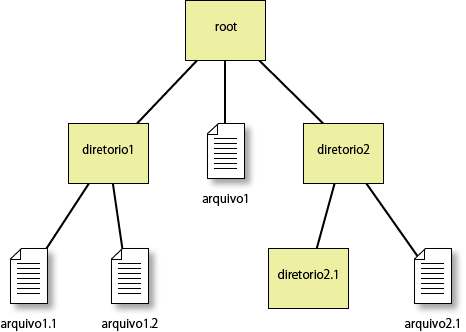
\includegraphics[clip,width=10.0cm]{images/image3.png}
			\caption{Árvore de diretórios}
			\label{fig:arv_dir}
		\end{center}
	\end{figure}
	
	\subsection{Serviço de Nomes}
	O serviço de nomes se preocupa em indicar a localização de um determinado arquivo, dado o seu nome ou caminho. Se a localização do arquivo estiver armazenada no nome dele, como por exemplo raiz/dir1/teste1, então esse serviço de nomes não provê transparência de localização. Para prover essa transparência, o nome ou caminho de um arquivo não deve ter indícios de sua localização física, e caso esse arquivo mude de lugar, ou tenha várias cópias, o seu nome ou caminho não precisará
	ser alterado para poder ser encontrado. Para isso, o serviço precisa oferecer ou resolução por nomes, ou resolução por localização, ou ambos.\\
	
	Resolução por nomes mapeia nomes de arquivos legíveis por humanos, normalmente \textit{strings}, para nomes de arquivos legíveis por computadores, que normalmente são números, facilmente manipuláveis pelas máquinas. Por exemplo, o endereço "www.endereco.com" ~ é mapeado para o IP 111.222.111.222. Através desse conjunto de números é possível encontrar uma máquina na rede IP, utilizando-se de tabelas de rotas de endereços mascarados que indicam como chegar à posição desejada.\\
	
	Resolução por localização mapeia nomes globais para uma determinada localização. Por exemplo, números de telefone, onde temos código do país, da localidade, etc. Se transparência por nome e por localização estiverem sendo utilizadas, pode ser muito difícil realizar um roteamento para determinar a localização de um determinado nome. Pode-se pensar em soluções com servidores
	centralizados ou distribuídos, porém os centralizados podem se tornar um gargalo, enquanto os distribuídos precisam usar alguma técnica de descentralização, como por exemplo cada servidor é responsável por um determinado subconjunto de arquivos, ou cada um cuidaria de resolver a localização de determinados tipos de arquivos, etc.
	
	%texto.... referência \cite{borsley96}
		

	\section{Conclusões do Capítulo}
Neste capítulo foi introduzido o que é um sistema de arquivos distribuído. De modo didático, primeiro foi explanado o que é um sistema distribuído, o que são metadados, e então, foi apresentado a definição e características de um sistema de arquivos distribuído.
 

	


%\chapter{Desenvolvimento}
\chapter{Computação na Nuvem}
	

 

	


\section{Resumo}
Este capítulo detalha o BFT-SMaRt apresentando seu conceito, princípios de Design, protocolos centrais, reconfiguração, implementação, configurações alternativas e finalizando nas conclusões do capítulo.


%	\section{BTF-SMART}
	\section{Conceitos}
	Na área da computação, a  replicação de máquina de estado (SMR), é um método para implementação de um serviço tolerante a falha em que um conjunto de servidores trabalham coordenadamente na interação com a máquina cliente e o serviço está implantado neste conjunto em vez de  apenas um. \\
	
	O BFT-SMART é uma biblioteca \textit{open-source} criado recentemente em linguagem Java que possui um conjunto de classes para implementar um sistema distribuído robusto consistindo de replicação de máquina de estado tolerantes a falhas bizantinas (falha bizantina ocorre quando uma máquina apresenta um comportamento arbitrário fora de sua especificação, por exemplo, quando um servidor é invadido e começa a rodar código malicioso) e apresentando confiabilidade, modularidade, reconhecimento de sistema multicore, suporte à reconfiguração e interface flexível de programação, como foi apresentado por Alchieri et al em \cite{bessani3}. \\
	
	Novamente em \cite{bessani3} é discutido como nos últimos anos a discurção sobre \textit{State Machine Replication (SMR)} tolerantes a falhas bizantinas (\textit{Byzantine Fault-Tolerant - BFT}) tem se acirrado contendo pouco avanço prático, apenas protótipos usados para validar ideias apresentadas em artigos, assim dificultando a aplicação dessa prática em aplicações reais. Os autores acreditam que isto seja devido à falta de implementações de um SMR BFT robusto. O BFT-SMaRt foi proposto tendo em mente contornar tal dificuldade, o qual almeja tanto alta performance em execuções livre de falhas quanto corretude mesmo com replicas que apresentam comportamento arbitrário. Incluindo o desenvolvimento de protocolos para transmissão de estados e reconfiguração. \\
	
	\section{Princípios do Design}
	
	%\begin{itemize}
		%\item Modelo Harmonioso de Falhas\\
		\subsection{Modelo Harmonioso de Falhas}
		BFT-SMaRt tolera falhas bizantinas não-maliciosas por padrão. Num modelo de sistema realistas mensagens podem ser enviadas, rejeitadas ou corrompidas, enquanto processos podem executar de forma anormal sem que ajam terceiros envolvidos. Além disso, também é possível configurar o BFT-SMaRt para que ele lide com falha bizantinas maliciosas, para tal ele provem assinaturas criptografadas. \\
		
		%\item Simplicidade\\
		\subsection{Simplicidade}
		A enfâse na corretude dos protocolos levou aos projetistas evitarem otimizações no código-fonte que poderiam acarretar em complexidade desnecessária tanto em tempo de desenvolvimento ou codificação. Este foi um dos motivos para a bibioteca ter sido desenvolvida em Java ou invés de outra slinguagends de programação em alto nível, como C/C++ ou Python.\\
		
		%\item Modularidade\\
		\subsection{Modularidade}
		BFT-SMaRt implementa um protocolo SMR modular que utiliza uma, bem definida, primitiva de consenso. Além de módulos responsáveis por garantir uma comunicação point-to-point confiável, ordenação de solicitações de clientes e o consenso entre SMRs, o BFT-SMaRt também implementa módulos de transferência de estados e reconfiguração, os quais são totalmente separados do protocolo de agreement.\\
		
		\begin{figure}[htb]
			\begin{center}
				
				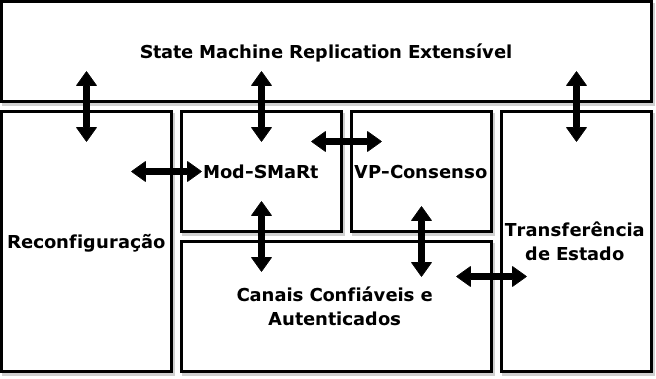
\includegraphics[clip,width=13.0cm]{images/image4.png}
				\caption{A modularidade do BFT-SMaRt. Adaptado de Alchieri~\cite{bessani3}}
				\label{fig:vis_sis}
			\end{center}
		\end{figure}
		
		%\item  Interface de Programação de Aplicação Simples e Extensível\\
		\subsection{Interface de Programação de Aplicação Simples e Extensível}
		A biblioteca java encapsula toda a complexidade do SMR BFT dentro de uma API que pode ser utilizada para a implementação de serviços determinísticos, utilizando métodos invoque(comando) para enviar comandos às réplicas quem implementam o método execute(comando) para que as réplicas processem o comando enviado. Entretanto, caso a aplicação necessite de comportamentos especializados não suportado por este modelo de programação, é possível utilizar outras chamadas ou plug-ins tanto no lado do cliente quanto do servidor.\\
		
		
		%\item Consciência de ambiente Multi-Core\\
		\subsection{Consciência de ambiente Multi-Core}
		BFT-SMaRt é capaz de aproveitar a arquitetura multicore dos servidores para diminuir o tempo de processamento em regiões críticas do protocolo.\\
		
		%\item Modelo do Sistema\\
		\subsection{Modelo do Sistema}
		BFT-SMaRt assume o modelo usual para sistemas BFT SMR: n $\geq$ 3f+1 réplicas para tolerar f falhas bizantinas. Entretanto, visto que o sistema suporta reconfiguração, é possível modificar n e f em tempo de execução. Além disso, o sistema permite ser configurado para utilizar apenas n $\geq$ 2f+1 réplicas para tolerar f falhas de sistema. Porém, independente da configuração, o sistema necessita de conexões point-to-point confiáveis entre os processos de comunicação. Essa conexão é realizada utilizando message authentication code (MAC) sobre o protocolo TCP/IP.\\
	%\end{itemize}
	
	\section{Protocolos Centrais}
	
	%\begin{itemize}
		%\item Total Order Multicast\\
		\subsection{Total Order Multicast}
		Em um sistema distribuído, um total order é um protocolo de mensagem broadcast que garante a entrega das mensagens de forma confiável e na mesma ordem para todos os participantes.\\
		
		Total Order Multicast é possível graças ao Mod-SMaRt, um protocolo modular que implementa BFT SMR utilizando uma primitiva de consenso. Durante sua fase de execução normal, a qual ocorre na ausência de falhas e na presença de sincronismo entre as outras réplicas, clientes enviam suas solicitações para todas as réplicas e aguardam pela resposta. Total order é alcançado através de uma sequência de instancias de consenso, cada uma delas decidindo sobre um lote de solicitações de clientes. Cada instância é composta por três passos de comunicação. O primeiro passo solicita que o líder do consenso envie uma mensagem de PROPOSE para cada réplica. Esta etapa é seguida por duas etapas de mensagens de todos para todos (all-to-all) compostas de mensagens WRITE e ACCEPT. Onde as mensagens de PROPOSE contém o lote de solicitações, WRITE e ACCEPT contém o hash criptografado de tal lote.\\
		
		Quando uma falha ocorre ou alguma replica encontra-se dessincronizada das demais, o Mod-SMaRt pode mudar de fase para a de sincronização. Durante esta fase um novo líder é eleito e as réplicas são forçadas a entrarem na mesma instância de consenso. Este “pulo” pode causar com que algumas réplicas ativem o protocolo de transferência de estados.\\
		
		%\item Transferência de Estado\\
		\subsection{Transferência de Estado}
		A fim de implementar uma SMR que possa ser usada na prática, faz-se necessário que as réplicas possam ser reparadas e reintegradas ao sistema sem que todo o sistema de replicação seja reiniciado. Para garantir tal característica, o BFT-SMaRt implementa algumas ideias chaves: (1) armazenar o log dos lotes de operações em execução em apenas um disco, (2) tirar snapshots em diferentes pontos da execução em várias réplicas e (3) realizar transferência de estados  de forma colaborativa, cada réplica enviando diferentes partes do estado para a réplica que está sendo recuperada.\\
	%\end{itemize}
	
	\section{Reconfiguração}
	BFT-SMaRt provem um protocolo especial que permite que réplicas sejam adicionadas ou executadas on-the-fly. Porém, tal processo só pode ser iniciado pelos administradores executando um cliente View Manager, por motivos de segurança.\\
	
	\section{Implementação}
	BFT-SMaRt foi desenvolvido contendo menos de treze mil e quinhentas linhas de código Java distribuídos em cerca de noventa arquivos. Tal característica é significativamente menor do que ocorre em sistemas similares que geralmente possuem mais de vinte mil linhas de código. \\
	
	Um ponto chave quando se está implementando um \textit{middleware} de replicação de alta vazão é como separar as várias tarefas do protocolo em uma arquitetura que seja eficiente e robusta. No caso de um \textit{Bizantine Fault Tolerante State Machine Replication} (BFT SMR) existem dois requisitos adicionais: o sistema precisa lidar com centenas de clientes e resistir a possíveis comportamentos maliciosos tanto dos clientes quantos das outras replicas.\\
	
	A Figura \ref{fig:image5} apresenta a arquitetura central com as \textit{threads}  usadas para o processamento das mensagens arquitetadas pela implementação do protocolo. Nesta arquitetura, todas as \textit{threads} comunicam através de filas delimitadas. A figura também mostra qual \textit{thread} alimenta e consume informações de cada fila. \\  
	
	\begin{figure}[htb]
		\begin{center}
			
			\includegraphics[clip,width=13.0cm]{images/image5.png}
			\caption{Processamento de mensagens arquitetadas entre replicas do BFT-SMaRt. Adaptado de Alchieri~\cite{bessani3} }
			\label{fig:image5}
		\end{center}
	\end{figure}
	
	As solicitações dos clientes são recebidas através da \textit{thread pool} provida pelo \textit{Netty Communitation Framework}. Assim que uma mensagem proveniente do cliente é recebida, é verificado se trata-se de uma solicitação ordenada ou não ordenada. Solicitações não ordenadas, as quais são geralmente aplicadas por comandos de apenas leitura, são entregadas diretamente para o serviço de implementação. No caso de uma solicitação ordenada, elas são entregues para o \textit{client manager}, o qual verifica a integridade da solicitação, caso esteja integra, a solicitação é encaminhada para a fila do respectivo cliente. Perceba que o endereço MAC dos clientes são verificados pelo \textit{Netty threads}, desta forma as maquinas multi-core e multi-processadas vão naturalmente aproveitar de seu poder para conquistar uma alta vazão. \\ 
	
	O \textit{proposer thread} é responsável por juntar um \textit{batch} de solicitações e transmitir a mensagem \textit{PROPOSE} do protocolo de consenso. O BFT-SMaRt preenche o \textit{batch} com solicitações pendentes até que: (a) seu tamanho alcance o máximo definido no arquivo de configuração; ou (b) não haja mais solicitações sobrando para serem adicionadas. Esta \textit{thread} só está ativa na replica líder. \\
	
	Cada mensagem \textit{m} que deve ser enviada de uma replica para outra é colocada na fila de saída (\textit{out queue}) pela qual uma \textit{sender thread} vai serializar a mensagem \textit{m}, produzir o endereço MAC que será anexado na mensagem e, enfim, enviar utilizando \textit{sockets TCP}. Do ponto de vista da replica que irá receber a mensagem, uma \textit{receiver thread} vai ler \textit{m}, autenticar (validar seu MAC), deserializar e colocar na fila de entrada (\textit{in queue}), onde todas as mensagens recebidas de outras replicas são armazenadas em ordem para serem processadas.  \\
	
	O \textit{message processor thread} é responsável por processar as mensagens provenientes do protocolo BFT SMR. Esta \textit{thread} carrega as mensagens da fila de entrada e as processa caso elas façam parte do consenso que está sendo executado, entretanto, caso a mensagem pertença a um consenso que ainda será executado, ela é processada posteriormente, quando seu consenso estiver ativo. Caso a mensagem não se encaixe em nenhum dos dois cados, ela é apenas descartada. \\
	
	 Quando um consenso chega ao fim em uma replica, ele é marcado como decidido e o \textit{batch} que o possui também o é marcado como decidido e colocado na fila de decididos (\textit{decided queue}). Então, o \textit{delivery thread} é chamado para coletar os \textit{batchs} que estejam armazenados nesta fila, deserializar todas as solicitações do \textit{batch}, remover cada uma delas das filas de seus respectivos clientes e marcar o  consenso corrente como finalizado. Após isso, o \textit{delivery thread} invoca o serviço de replica (\textit{service replica}) para executar a solicitação e gerar a reposta correspondente. Quando terminar de gerar a resposta, o serviço de replica a adiciona na fila de resposta (\textit{reply queue}). O \textit{reply thread} carrega as respostas armazenadas nessa fila e as manda para seus referidos clientes. \\
	 
	 O \textit{request timer thread} é ativado periodicamente afim de verificar se alguma solicitação permanece como não respondida por mais tempo do que o delimitado por um tempo de \textit{timeout} predefinido em alguma fila de solicitações (\textit{requests queue}). A primeira vez que este \textit{timer} expira para alguma solicitação, faz com que esta solicitação seja encaminhada para o líder corrente. A segunda vez que este \textit{timer} expira para a mesma solicitação, a instância atual do protocolo de consenso é paralisado a fase de sincronização é ativada. A base lógica destes \textit{timers} é a seguinte: em uma rede em condições normais, o \textit{timeout} pode ser causado por algum cliente que não enviou a solicitação ao líder ou pelo líder que não encaminhou os pedidos das solicitações dos clientes. Visto que tipicamente existem muitos clientes para poucos servidores, é esperado que ocorra mais falhas no lado dos clientes do que dos servidores, por isto o protocolo do BFT-SMaRt assume que o erro ocorreu no lado do cliente, sendo que suspeita-se do líder somente se o problema persistir. \\
	 
	 \section{Configurações Alternativas}
	 
	 Como mencionado nas seções anteriores, por padrão o BFT-SMaRt tolera falhas bizantinas não maliciosas. Entretanto, o sistema pode ser configurado para suportar dois outros modelos de falhas.\\
	 
	 %\begin{itemize}
	 	%\item \textit{Crash Fault Tolerance} \\
	 	\subsection{\textit{Crash Fault Tolerance}}
	 	BFT-SMaRt suporta uma configuração de um parametro que caso seja ativado faz com que o sistema tolere apenas falhas de \textit{crash}. Quando esta propriedade está ativa, o sistema tolera  f \textless  n/2 (minoria simples), o que implica alterações em todos os passos necessários do protocolo, inclusive ignorando o passo do \textit{WRITE} durante a execução do consenso. Fora essas alterações, o protocolos é o mesmo do caso de tolerância de falha bizantina. 
	 	
	 	%\item Falhas Bizantinas Maliciosas\\
	 	\subsection{Falhas Bizantinas Maliciosas}
	 	Trabalhos anteriores ao BFT-SMaRt demonstraram que o uso de assinaturas com chaves públicas sobre solicitações torna impossível para os clientes forjarem vetores MAC e força que o líder seja alterado. Por padrão, o BFT-SMaRt não utiliza assinaturas de chave pública além da utilizada para estabelecer chaves simetricas compartilhadas entre replicas e durante a mudança do líder. Contudo, o sistema opcionalmente permite o uso de solicitações assinadas para evitar esse problema.\\
	 	
	 	Os mesmos trabalhos também mostram que líderes maliciosos podem lançar ataques de degradação de performance indetectáveis , fazendo com que a vazão do sistema caia drasticamente. Até o presente momento, o BFT-SMaRt não apresenta meios de defesa conta este tipo de ataque. \\
	 	
	 	Por fim, o fato do BFT-SMaRt ter sido desenvolvido em Java faz com que seja fácil aplicar o sistema em diferentes plataformas. Esta escolha permitiu que o time de desenvolvimento evitasse falhas de um unico nó causadas por eventos acidentais (por exemplo, algum \textit{bug} ou problemas de infraestrutura) or ataques maliciosos aproveitando de vulnerabilidades comuns.  \\
	 %\end{itemize}
	   
	
	%texto.... referência \cite{borsley96}
		
		\section{Conclusões do Capítulo}
	Neste capítulo foi detalhado o BFT-SMaRt apresentando seu conceito, princípios de Design, protocolos centrais, reconfiguração, implementação, configurações alternativas.
\chapter{RAID}
Neste capítulo é apresentado os conceitos do que é RAID e quais são as peculiaridades de suas principais categorias. O capítulo está dividido em duas seções, na primeira é apresentado os conceitos de RAID separado em subseções para os tipos RAID 0, RAID 1, RAID 2, RAID 3, RAID 4, RAID 5, RAID 6 e RAID 50. Finalmente, o capítulo termina com a seção de conclusões do capítulo.

%	\section{RAID}
		\section{Conceitos}
		O desempenho da unidade de processamento e da memória principal cresceu rapidamente. Para se ter uma ideia do tamanho do crescimento espetacular de desempenho destes componentes, entre os anos de 1974 e 1984 a performance deles aumentava em 40\% por ano, cerca de duas vezes maior do que a frequência geral dos microcomputadores. Deste modo uma instrução de CPU do tipo entrada/saída (E/S) tem a possibilidade de se tornar um grande gargalo, devido que o desenvolvimento do dispositivo de armazenamento magnético, em questão de velocidade de acesso, não acompanha o crescimento dos dois componentes principais, o processador e a memória.\\
		
		O RAID, originalmente a sigla do \textit{redundant array of inexpensive disk}, mas atualmente é mais conhecido como \textit{redundant array of independent disk}.Seu princípio é uso de disco extra para a recuperação da informação original em caso de uma falha num disco. Em ~\cite{patterson88} Patterson \textit{et al} demonstrou que sem um controle de tolerância à falhas, grandes \textit{arrays} de discos baratos não podem ser considerados uteis devido a sua baixa taxa de confiabilidade. A proposta inicial de Patterson \textit{et al} ao desenvolver o RAID era de que para superar o obstaculo da falta de confiabilidade era necessário o uso de discos extras que possuíssem informação redundante que possibilitassem a recuperação total das informações originais no caso da falha de algum disco. Vale resaltar que a proposta inicial do RAID foi desenvolvida utilizando como referencia o \textit{hardware}, contudo, Petterson emseu artigo original ~\cite{patterson88} frisa que as ideias centrais do projeto poderiam ser aplicadas facilmente na implementação de\textit{softwares}, e este ponto é de fundamental importância para nosso trabalho. Sendo que a ideia central apresentada por Patterson era de quebrar os \textit{arrays} em grupos confiáveis, onde cada grupo possua discos extras possuidores de informação redundante que seriam utilizados para manter a previamente citada confiabilidade dos grupos. De forma que quando um disco falhar, em um espaço curto de tempo o disco faltoso será substituído por um novo disco e a informação que estava contida no antigo disco será totalmente reconstruída no novo utilizando as informações redundantes contida no grupo. Este tempo de espera ficou conhecido como \textit{mean time to repair (MTTR)} ou em uma tradução livre, "tempo de conserto". O MTTP pode ser reduzido se o sistema possuir discos extras que funcionem como peças sobressalentes em estado de prontidão de forma que quando um disco falha, ele é trocado por um desses discos extras de forma eletrônica, sem que haja a necessidade de intervenção humana (bastando apenas que de tempos em tempos, um técnico humano troque os discos defeituosos por novos discos extras). Patterson, ao desenvolver o conceito de RAID, assumiu que as falhas de discos são independentes e exponenciais (sendo que no caso de um desastre natural ou da falta inesperada de alimentação são situações em que a falha de vários discos não seja independentes). \\
		
		O RAID é separado em diferentes níveis, sendo que cada nível possuiu seus objetivos distintos e características intrínsecas. Os principais níveis de RAID serão apresentados e explicados nas próximas subseções deste trabalho. Cada subseção subsequente será dedicada a um nível de RAID.\\
		
		\subsection{RAID 0}
		
		Também conhecido como \textit{Strinping} ou fracionamento, pois os dados são fracionados igualmente entre dois ou mais discos, sem a preocupação com informação de paridade, tolerância a falhas ou redundância. Devido ao fato da completa falta de tolerância a falhas no RAID 0, a perda de um disco acarreta na perda (sem qualquer chance de recuperação) de todos os dados contidos no disco e da inutilização de todas as outras frações dos dados que estavam armazenadas nos outros discos do vetor, visto que estes arquivos jamais serão completamente recuperados. Por esta razão que o RAID 0 é usado apenas nos casos em que se deseja aumentar a performance do sistema ou como forma de criar uma grande unidade lógica de armazenamento utilizando-se dois ou vários discos físicos. Inclusive, é possível modelar um sistema em RAID 0 utilizando-se discos de diferentes capacidades, entretanto, é importante frisar que os discos com maior quantidade de armazenamento disponível serão limitados ao espaço máximo do menor disco do vetor, por exemplo, em um vetor montado com dois discos, um com 500GB e um segundo de 280GB possuirá o total de 560GB de armazenamento, ou seja, 280 X 2, nitidamente o disco de 500GB está sendo subutilizado neste vetor. \\
		
		A figura ~\ref{fig:raid0} representa o diagrama de um vetor modelado com o RAID 0 utilizando-se dois discos. Visto que os dados contidos nos discos 0 e 1 podem ser recuperados simultaneamente resulta na ilusão de que o \textit{drive} é mais rápido.\\
		
		\begin{figure}[htb]
			\begin{center}
				
				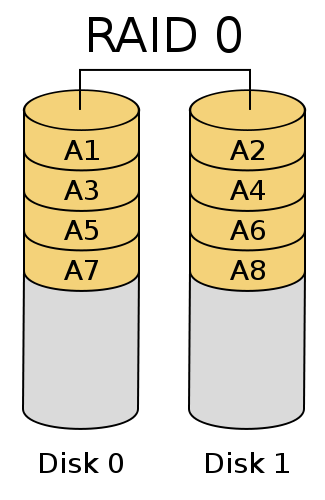
\includegraphics[clip,width=6.0cm]{images/RAID_0.png}
				\caption{Diagrama do RAID 0. Retirado da Wikipedia~\citep{wikiRAIDlevels}.}
				\label{fig:raid0}
			\end{center}
		\end{figure} 
		
		\subsubsection{Performance}
		
		RAID 0 pode ser usado em áreas onde a performance é crucial enquanto que a integridade dos dados é de pouca relevância, como ocorre no caso dos sistemas de jogos de video game online.\\
		
		\subsection{RAID 1}
		
		RAID 1 é também conhecido como \textit{mirror} ou espelhamento, visto que este nível consiste de uma copia exata de um conjunto de dados espalhado por dois ou mais discos. A configuração do RAID 1 não proporciona paridade ou fracionamento de dados, visto que os dados são apenas espelhados dentro de todos os discos pertencentes do vetor de discos, sendo que o espaço de armazenamento do vetor não pode ser maior do que o disco membro com o menor espaço de armazenamento. O vetor continuará funcional enquanto ao menos um membro do vetor esteja disponível. Esta configuração é útil para sistemas onde a confiança e performance de leitura é mais importante do que performasse de escrita ou um armazenamento eficiente. \\
		
		A figura ~\ref{fig:raid1} representa o diagrama de um vetor modelado com o RAID 1 utilizando-se dois discos.\\
		
		\begin{figure}[htb]
			\begin{center}
				
				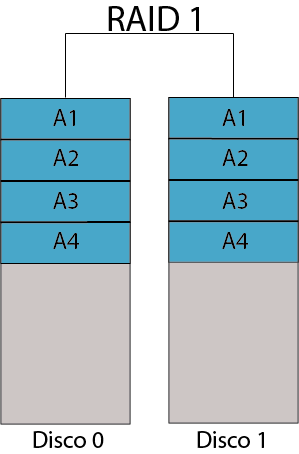
\includegraphics[clip,width=6.0cm]{images/RAID_1.png}
				\caption{Diagrama do RAID 1. Retirado da Wikipedia~\citep{wikiRAIDlevels}.}
				\label{fig:raid1}
			\end{center}
		\end{figure} 
		
		\subsubsection{Performance}
		
		Qualquer solicitação pode ser atendida por qualquer \textit{drive} no vetor. Sendo que no caso de solicitações de escrita o desempenho é comprometido pois é necessário que ela ocorra em todos os discos membros do vetor. \\
		
		\subsection{RAID 2}
		
		A configuração RAID 2 fraciona o dado ao nível do \textit{bit} ao invés de blocos, além de utilizar a técnica do Código de Hamming para a correção de erros. O eixo de rotação de todos os discos são sincronizados e o dado é fracionado de forma que cada sequência de \textit{bits} são armazenadas em discos diferentes. A paridade do código de hamming é calculada sobre os \textit{bits} correspondentes e armazenadas em ao menos um disco de paridade.\\
		
		A figura ~\ref{fig:raid2} representa o diagrama de um vetor modelado com o RAID 2 utilizando-se sete discos, sendo três deles utilizados como discos de paridade.\\
		
		\begin{figure}[htb]
			\begin{center}
				
				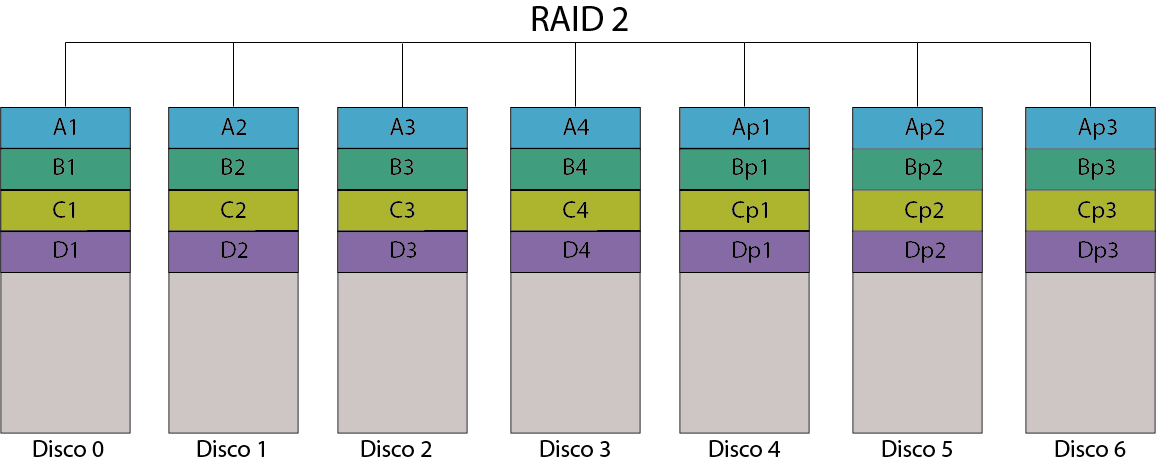
\includegraphics[clip,width=10.0cm]{images/RAID_2.png}
				\caption{Diagrama do RAID 2. Retirado da Wikipedia~\citep{wikiRAIDlevels}.}
				\label{fig:raid2}
			\end{center}
		\end{figure} 
		
		\subsubsection{Performance}
		Por utilizar o código de Hamming, possui forte tolerância a falhas. Entretanto, como os discos rígidos atualmente possuem correção interna de erros, o RAID 2 acabou perdendo seu propósito. 
	
	
		\subsection{RAID 3}
		
		Diferente do RAID 2, o RAID 3 fraciona os dados ao nível do \textit{byte}, tendo um disco dedicado de paridade. O eixo de rotação de todos os discos são sincronizados e o dado é fracionado de forma que cada sequência de \textit{bytes} são armazenadas em discos diferentes. A paridade é calculada sobre os \textit{bytes} correspondentes e armazenadas no disco de paridade. Apesar de existir casos de implementação, o RAID 3 dificilmente é utilizado na prática.\\
		
		A figura ~\ref{fig:raid3} representa o diagrama de um vetor modelado com o RAID 3 utilizando-se quatro discos, sendo um deles utilizados como disco de paridade.\\
		
		\begin{figure}[htb]
			\begin{center}
				
				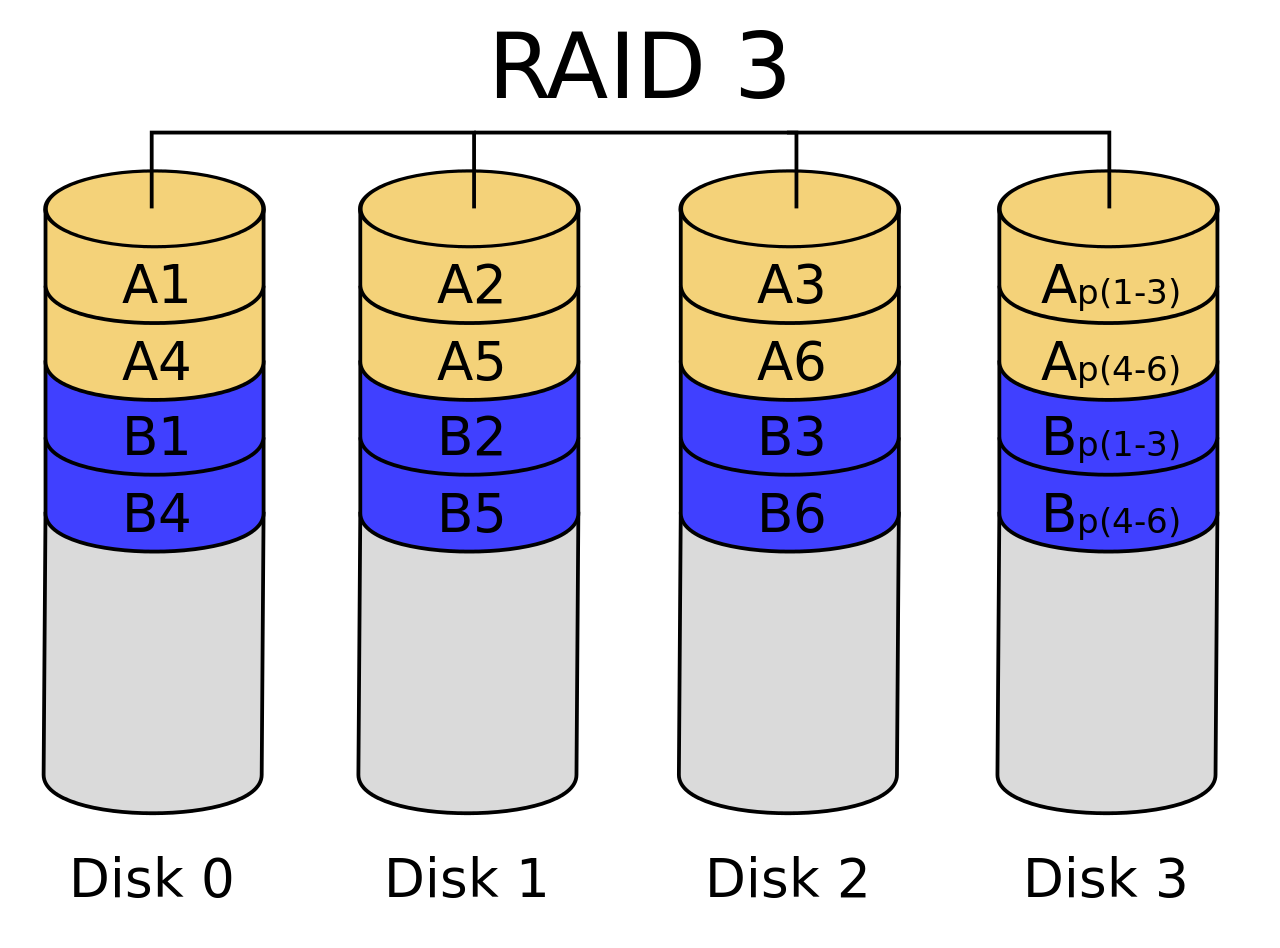
\includegraphics[clip,width=10.0cm]{images/RAID_3.png}
				\caption{Diagrama do RAID 3. Retirado da Wikipedia~\citep{wikiRAIDlevels}.}
				\label{fig:raid3}
			\end{center}
		\end{figure} 
		
		\subsubsection{Performance}
		Esta configuração se encaixa para aplicações que necessitam de altas taxas de transferência de grandes sequências de dados sequenciais, como por exemplo, edição de vídeos não compressados. Todavia, aplicações que fazem uso de leituras e escritas em localizações aleatórias do disco tendem a ter uma performance sofrível, visto que as frações de um mesmo dado estão espalhadas nas mesmas seções dos vários discos do vetor.\\
		
		\subsection{RAID 4}
		Diferente dos RAID 2 e 3, o RAID 4 fraciona os dados ao nível do bloco de dados, tendo um disco dedicado de paridade. \\
		
		A figura ~\ref{fig:raid4} representa o diagrama de um vetor modelado com o RAID 4 utilizando-se quatro discos, sendo um deles utilizados como disco de paridade.\\
		
		\begin{figure}[htb]
			\begin{center}
				
				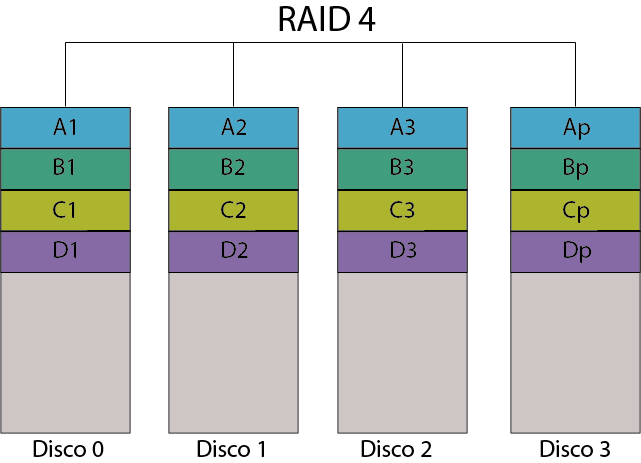
\includegraphics[clip,width=10.0cm]{images/RAID_4.png}
				\caption{Diagrama do RAID 4. Retirado da Wikipedia~\citep{wikiRAIDlevels}.}
				\label{fig:raid4}
			\end{center}
		\end{figure} 
		
		\subsubsection{Performance}
		Sempre que os dados são escritos no vetor, o novo dado sobre paridade deve ser recalculado e escrito para o respectivo disco de paridade antes que qualquer requisição de escrita seja realizada. Por causa dessas operações de leitura e escrita, o disco de paridade é o fator limitante do desempenho total do vetor.\\
		
		\subsection{RAID 5}
		Similar ao RAID 4, o RAID 5 fraciona os dados ao nível do bloco de dados, porém tendo as informações de paridade espalhadas entre os discos do vetor. Isto exige que todos, exceto um, discos tenham os dados. No caso da falha de apenas um disco, leituras subsequentes podem ser calculadas utilizando-se os dados restantes e (caso o disco defeituoso não seja o que continha os dados de paridade do arquivo) das informações de paridade para recuperar o bloco faltoso de dados. Entretanto, caso o disco que está indisponível é o portador dos dados de paridade, não acarreta na necessidade de nenhum calculo a mais. É importante frisar que por suas características, o RAID 5 necessita de ao menos três discos.  \\
		
		A figura ~\ref{fig:raid5} representa o diagrama de um vetor modelado com o RAID 5 utilizando-se quatro discos.\\
		
		\begin{figure}[htb]
			\begin{center}
				
				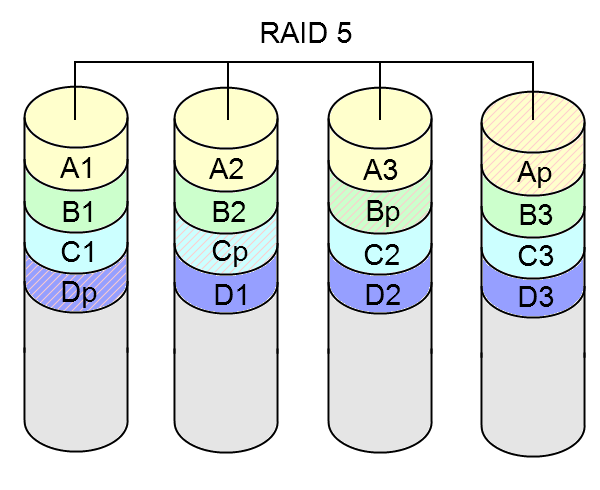
\includegraphics[clip,width=10.0cm]{images/RAID_5.png}
				\caption{Diagrama do RAID 5. Retirado da Wikipedia~\citep{wikiRAIDlevels}.}
				\label{fig:raid5}
			\end{center}
		\end{figure} 
		
		\subsubsection{Performance}
		O RAID 5 sofre pelo tempo demasiadamente grande necessário para reconstruir um arquivo a partir dos blocos restantes e do bloco de paridade, além da chance de mais um disco ficar indisponível durante a a fase de recuperação. Visto que a recuperação de um bloco de dados requer a leitura de todos os blocos de dados, abrindo a chance de perder todos os dados do vetor caso ocorra a perda de um segundo disco.\\
		
		\subsection{RAID 6}
		Similar ao RAID 5, o RAID 6 fraciona os dados ao nível do bloco de dados, porém tendo as informações de paridade espalhadas entre os discos do vetor e duplicadas. A novidade da paridade dupla garante tolerância a falhas até o caso da perda de dois discos. RAID 6 exige a utilização de no mínimo quatro discos. \\ 
		
		Semelhante ao caso do RAID 5, a queda de um disco acarreta na redução da performance de todo o vetor até que o disco defeituoso tenha sido substituído.\\

		
		A figura ~\ref{fig:raid6} representa o diagrama de um vetor modelado com o RAID 6 utilizando-se cinco discos.\\
		
		\begin{figure}[htb]
			\begin{center}
				
				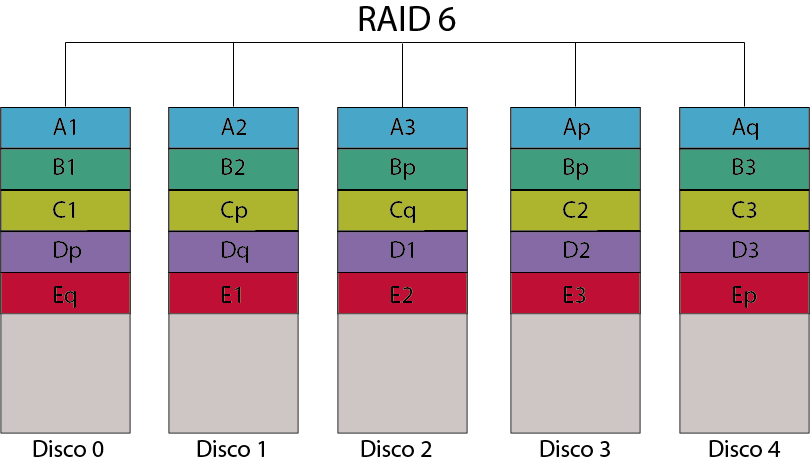
\includegraphics[clip,width=10.0cm]{images/RAID_6.png}
				\caption{Diagrama do RAID 6. Retirado da Wikipedia~\citep{wikiRAIDlevels}.}
				\label{fig:raid6}
			\end{center}
		\end{figure} 
		
		\subsubsection{Performance}
		RAID 6 não possui penalidade de performance sobre operações de leitura, contudo, possui penalidade de performance nas operações de escrita devido ao \textit{overhead} associado aos cálculos de paridade.\\
		
		
		\subsection{RAID 50}
		Existe o termo originalmente conhecido como RAID hibrido, o qual é definido pela aplicação de um nível de RAID sobre outro vetor formado por nível de RAID. O ultimo vetor gerado é conhecido como o 
		vetor do topo. Logo, no caso do RAID 50 (ou RAID 5+0) é uma combinação híbrida que usa as técnicas de RAID 5 com paridade em conjunção com a segmentação de dados do RAID 0. Em outras palaras, o RAID 50 não passa da aplicação do RAID 0 sobre um vetor de RAID 5. \\
		
		A figura ~\ref{fig:raid50} representa o diagrama de um vetor modelado com o RAID 50 utilizando-se três conjuntos de três discos cada.\\
		
		\begin{figure}[htb]
			\begin{center}
				
				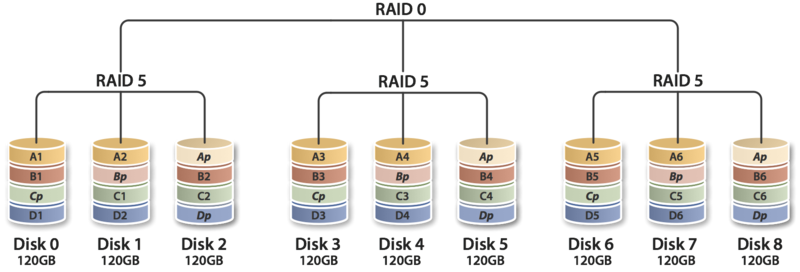
\includegraphics[clip,width=15.0cm]{images/RAID_50.png}
				\caption{Diagrama do RAID 50. Retirado da Wikipedia~\citep{wikiRAIDlevels}.}
				\label{fig:raid50}
			\end{center}
		\end{figure} 
		
		\subsubsection{Performance}
		Possui alta taxa de transferência, porém com alto custo de manutenção e expansão.
		
	%texto.... referência~\citep{patterson88}
	
	\section{Conclusões do Capítulo}
	Neste capítulo foi apresentado os conceitos de básicos do que é RAID, suas características positivas e negativas, além de abordar sobre as topologias mais importantes do RAID, ou seja, RAID 0, RAID 1, RAID 2, RAID 3, RAID 4, RAID 5, RAID 6 e RAID 50.
		



 

	


\chapter{Proposta de Sistema de Arquivos Distribuído}
Este capítulo é onde começamos a abordar nosso modelo proposto de um sistema de arquivos distribuídos tolerante a falhas. Iniciamos com um visão geral da arquitetura do sistema apresentando detalhes do serviço de metadados, serviço de armazenamento, servidor e do cliente. Em seguida é abordado as operações realizadas pelo sistema de arquivos distribuído proposto, tais operações estão divididas entre operações do tipo Cliente-Servidor e Servidor-Servidor. Seguindo com o capítulo, é explanado como foi realizada a implementação do sistema de arquivos distribuído utilizando conceitos de RAID, focando especialmente nos serviços de metadados e de armazenamento, além dos clientes. O capítulo finaliza apresentado o planejamento e execução dos experimentos seguido da análise dos dados obtidos.


	\section{Arquitetura do sistema}
	
	A arquitetura do Sistema de Arquivos Distribuídos proposto neste trabalho é composto por um ou vários clientes comunicando-se com servidores de metadados e servidores de armazenamento, onde cada um deles está conectado através de Internet ou outra rede, como a Figura~\ref{fig:vis_sis}  sintetiza. Neste sistema, cada servidor de armazenamento se comporta como um disco rígido em sistema de RAID, armazenando distribuidamente as partes dos arquivos e/ou paridades associadas. \\
	
	
	%O nosso objeivo neste artigo é a construção de um SAD baseado na computação em nuvem que possui menor \textit{overhead} de espaço, comparado a 200\% de método de replicação, sem degradar muito o performance e segurança de dados. 
	%Para isso, nós observamos em técnica de redundância usado na tecnologia RAID, onde consegue diminuir o espaço ocupado pela parte redundante com atribuição de paridade nos arquivos, ao invés de simples replicação. Na mesma tecnologia também foi 


\begin{figure}[htb]
	\begin{center}
		
		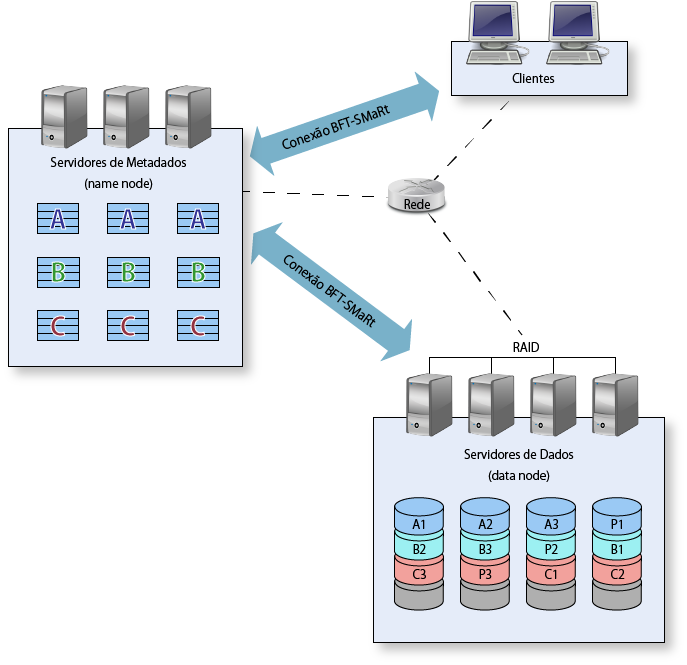
\includegraphics[clip,width=10.0cm]{images/visao_geral.png}
		\caption{Visão geral do sistema}
		\label{fig:vis_sis}
	\end{center}
\end{figure}

Em um sistema de arquivos local, normalmente o metadado e o conteúdo de um arquivo são armazenados na mesma unidade de armazenamento. No caso de um SAD, como um arquivo pode ser armazenado distribuidamente entre servidores diferentes, os metadados são espalhados por vários servidores, tendo assim, a necessidade de fazer a busca para acessar em um determinado metadado. Obviamente essa busca consome recursos operacionais, relativamente alta por tratar de uma transmissão na rede.
Além disso, os metadados devem ser mantidos de forma replicada para suportar falhas em algumas réplicas sem afetar a consistência do SAD.
   \\

%\begin{figure}[htb]
%	\begin{center}
		
%		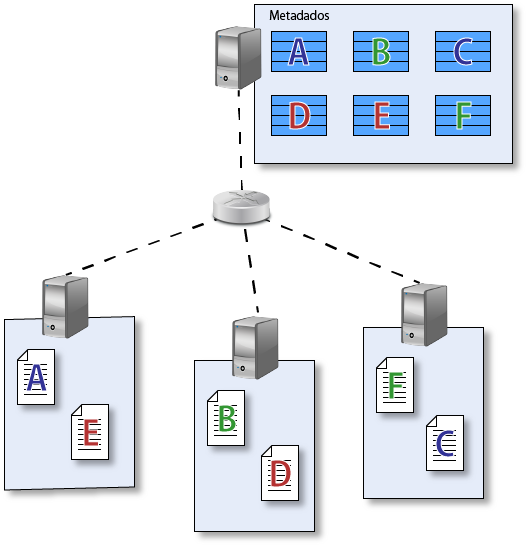
\includegraphics[clip,width=10.0cm]{images/image7.png}
%		\caption{\textit{Name node} e \textit{data node}}
%		\label{fig:namenode}
%	\end{center}
%\end{figure}

\subsection{Serviço de Metadados}
%Grupo de servidores que fazem o gerenciamento dos dados.\\

Em nosso sistema utilizamos o conceito de blocos, onde um bloco é um conjunto de dados de um dado arquivo ou os dados de paridade de um determinado arquivo. O tamanho do bloco é determinado levando em consideração a quantidade de servidores de armazenamento ativos, ou seja, se houverem quatro servidores ativos, então o arquivo (independente de seu tamanho) será dividido em quatro blocos de tamanhos idênticos, caso seja necessário, o último bloco será preenchido com bits "0" ~até que o bloco alcance o tamanho previamente fixado.
\\ 

O Serviço de metadados é o conjunto de servidores, chamados de \textit{name node}, que gerencia as informações dos arquivos armazenados, utilizando-se dos metadados. Em nosso sistema a data de criação, data da última modificação, data do último acesso, tamanho, identificador do bloco de dados e nome do servidor são considerados metadados. 
\\

É da responsabilidade do sistema de metadados gerenciar a comunicação entre cliente e servidores de armazenamento (ou  \textit{data nodes}), utilizando-se das informações que indicam o estado atual do sistema e qual o tipo de RAID está sendo utilizado (apenas um tipo de RAID pode ser utilizado por operação) o \textit{name node} deve decidir em quantos blocos de tamanho idêntico o arquivo deve ser dividido e em quais servidores de armazenamento cada bloco deve ser armazenado.
\\ 

Nosso sistema está preparado para tratar os seguintes tipos de RAID, os quais foram explorados com maior profundidade no Capítulo 4.
\\

\begin{itemize}
	\item RAID 0 - fracionamento simples;
	\item RAID 1 - espelhamento;
	\item RAID 5 - fracionamento com paridade espalhada entre os discos do vetor.
\end{itemize}

O Serviço de metadados mantém na sua memória local a árvore de diretórios, o que indica localização lógica dos arquivos. Quando recebe uma solicitação de cliente por um arquivo, pesquisa a sua árvore de diretórios para identificar qual diretório que este arquivo se encontra. Como resultado da pesquisa obtém os metadados do arquivo referente, conseguindo descobrir a sua localização física, a lista dos todos os \textit{data nodes} que possuem as partes do arquivo.
\\

Por sua propriedade como um interface entre clientes e \textit{data nodes}, a ocorrência de alguma falha na operação ou indisponibilidade causada pela queda do servidor tem  enorme influencia na execução do sistema, podendo até resultar em parada total do sistema. Assim, é muito importante elaborar uma esquema para manter o \textit{name node} protegidos contra falhas ou queda total. Em nosso sistema usaremos a biblioteca BFT-SMaRt, que fornece tolerância a falha no serviço através de replicação por máquina de estado~\citep{bessani3}. \\

\subsection{Serviço de Armazenamento}
Grupo de servidores responsáveis pelo armazenamento físico dos dados gerenciados pelo sistema de metadados. Também conhecido como \textit{data nodes}.
Em nosso sistema, o serviço de armazenamento não possui a necessidade de saber qual tipo de RAID está sendo executado, a responsabilidade de manter o RAID consistente é toda do serviço de metadados. Desta forma, o sistema de armazenamento apenas se conecta a uma porta e fica aguardando algum cliente se conectar a sua respectiva porta. Quando algum cliente conecta-se na porta do servidor, é realizado um \textit{handshake} preliminar, logo em seguida o cliente inicia a transferência dos dados que devem ser guardados pelo sistema de armazenamento. Ao fim da transferência o cliente fecha a conexão, enquanto o sistema de armazenamento indexa o arquivo recebido utilizando as informações adicionais que o serviço de metadados anexou ao arquivo. Com tais informações é possível saber o identificador tanto do arquivo quanto do cliente que o enviou. Tais dados adicionais são necessários para garantir que apenas o usuário dono dos dados enviados tenha acesso a eles, além de possibilitar identificar quais dados o cliente deseja receber de forma simples e eficiente.  
\\

\subsection{Cliente}
O programa cliente executado no computador do usuário final de nosso sistema. 
Para cada operação que deseje realizar, o programa cliente (doravante chamado Cliente) deve primeiramente comunicar-se com o serviço de metadados, o qual ou irá realizar a operação (no caso de operações envolvendo diretórios) ou informar com quais servidores de armazenamento o cliente deve se comunicar e quais blocos devem ser enviados para cada servidor (no caso de operações envolvendo arquivos). Entretanto, é função do Cliente informar qual tipo de RAID ele deseja utilizar.
\\

Após a comunicação inicial com o serviço de metadados, caso o cliente solicite pelo \textit{upload} ele deve iniciar a comunicação com os servidores de dados informados pelo serviço de metadados. Caso o cliente for utilizar o RAID 5, é ele quem fica responsável por calcular a paridade do arquivo, isto deve-se ao fato de que apenas o cliente conhece o arquivo. O procedimento para o calculo da paridade é exemplificado na figura~\ref{fig:img6}. Outra atribuição do cliente é fazer o particionamento do arquivo em blocos de iguais tamanhos, cada bloco será enviado para um dos servidores de dados informado pelo metadado, ou seja, o arquivo deve ser fragmentado de tal forma que cada servidor receba um bloco de dados, frisando que no caso do RAID 5 um dos blocos deve conter apenas informações de paridade previamente calculado pelo cliente. 
\\

\begin{figure}[htb]
	\begin{center}
		
		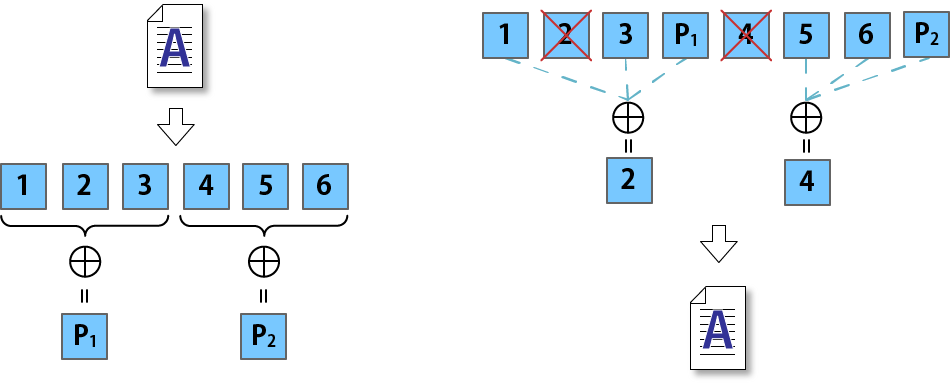
\includegraphics[clip,width=15.0cm]{images/image6.png}
		\caption{Geração de paridade}
		\label{fig:img6}
	\end{center}
\end{figure}

Caso a operação desejada pelo usuário final seja a de \textit{download} de algum de seus arquivos, o cliente deve coletar as informações de quais servidores possuem os blocos do arquivo almejado e quais as informações de identificação de cada bloco através do servidor de metadados. Com posse de tais informações, o cliente deve iniciar a comunicação com cada um dos servidores de dados apresentando a identificação de qual bloco cada servidor de dados deve enviar. Quando todos os servidores acabarem seus envios, o cliente deve usar os dados em sua posse para unir todos os blocos e recriar o arquivo desejado pelo usuário. Obviamente, esta descrição genérica da operação vai sofrer leves alterações dependendo de qual opção de RAID o cliente esteja utilizando. Para a opção de RAID 5, é possível que um dos blocos recebidos pelo cliente seja um bloco de paridade, para esse caso, o cliente deve utilizar as informações dos outros blocos para determinar qual é o bloco de dados faltante e utilizar a paridade para recuperar tal bloco. A Figura~\ref{fig:img2} mostra um esquema simplificado da operação de recuperar um arquivo realizado pelo lado do cliente.
\\

\begin{figure}[htb]
	\begin{center}
		
		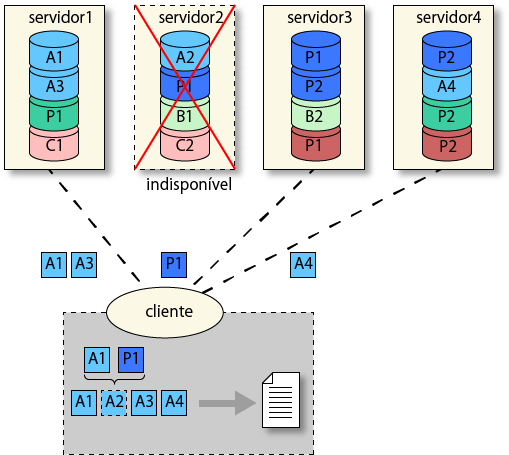
\includegraphics[clip,width=10.0cm]{images/image2.png}
		\caption{Recuperando um arquivo de uma falha}
		\label{fig:img2}
	\end{center}
\end{figure}

\section{Operações no Sistema de Arquivos Distribuídos}

Nesta seção serão apresentadas as operações básicas que o nosso SAD executa. Tais operações podem ser divididas em dois grupos dependendo das entidades envolvidas. O primeiro deles é entre cliente e servidor, composta por operações envolvendo solicitações de ações do cliente para o servidor. O segundo tipo são as operações que ocorrem entre servidores, voltadas para o gerenciamento do serviço sendo que este tipo de operações deve ocorrer de forma transparente para o cliente.
\\

\subsection{Cliente-Servidor}

É um conjunto de operações semelhantes as que são implementadas em um sistema de arquivos local, aquele que é integrado na maioria dos sistemas operacionais centralizados. Composto pelas operações sobre arquivos ou pastas, e suas execuções ocorrerem entre cliente e \textit{name node} ou \textit{data node}.

\subsubsection{Criar arquivo}

Operação realizada inicialmente entre o cliente e o servidor do tipo \textit{name node}. Nesse primeiro momento o cliente informa ao \textit{name node} que deseja criar um novo arquivo e em qual diretório ele deve ser criado, além de enviar os metadados do arquivo que pretende criar. Com posse dessas informações e de qual RAID está operando, o servidor de metadados processa e transmite para o cliente para quais \textit{data node} os blocos do arquivo devem ser enviados e qual a identificação de cada bloco. O processamento de tais informações é diretamente influenciado pelo estado atual do sistema, o \textit{name node} leva em consideração a disponibilidade de cada \textit{data node} e o quanto de espaço livre em disco que cada um possui.
\\

A segunda parte da operação é realizada entre o cliente e os servidores do tipo \textit{data node}. Após a comunicação com o servidor de metadados, o cliente sabe para quantos \textit{data nodes} o seu arquivo será enviado, desta forma, o cliente fragmenta o arquivo de forma que cada \textit{data nodes} irá receber um bloco de tamanho uniforme. Caso o sistema esteja usando o RAID 5, o cliente ainda deve calcular o bloco de paridade do arquivo e enviar para um dos \textit{data nodes}.
\\

\subsubsection{Criar diretório}

Operação realizada exclusivamente entre o cliente e o servidor \textit{name node}. Nessa operação o cliente informa ao \textit{name node} que deseja criar um diretório, passando como metadados apenas o nome do novo diretório e o nome de seu diretório pai. Com tais informações, o servidor de metadados primeiramente verifica se já existe um diretório com o mesmo nome no diretório pai, em caso negativo ele atualiza a árvore de diretório do cliente. No caso de já existir um diretório com mesmo nome, o cliente é informado e o novo diretório não é criado.
\\

\subsubsection{Abrir arquivos}

Operação realizada inicialmente entre o cliente e o servidor do tipo \textit{name node}. Nesse primeiro momento o cliente informa ao \textit{name node} que deseja abrir um arquivo, para tal, o cliente deve fornecer o nome do arquivo e o nome do diretório onde ele está. A primeira ação do servidor de metadados é verificar se o arquivo de fato existe no diretório informado, em caso positivo ele deve verificar se o cliente possui acesso ao arquivo. No caso do cliente possuir acesso, o \textit{name node} verifica em quantos blocos o arquivo foi dividido e em quais \textit{data nodes} cada bloco foi armazenado, após coletar tais informações, o servidor de metadados informa ao cliente quais servidores de dados ele, o cliente, deve se comunicar e o identificador de cada bloco. Para o caso de o arquivo não existir no diretório informado ou do cliente não possuir acesso para tal arquivo, o servidor de metadados deve enviar uma mensagem de erro informando a indisponibilidade do arquivo solicitado. 
\\

A segunda parte da operação é realizada entre o cliente e os servidores do tipo \textit{data node}. Após a comunicação com o servidor de metadados, o cliente sabe em quais \textit{data nodes} os blocos de seu arquivo estão armazenados. Desta forma, o cliente inicia a comunicação com cada \textit{data node} informado. A comunicação procede da seguinte forma, o cliente informa o identificador do bloco que deseja receber, enquanto que o \textit{data node} apenas verifica a existência do bloco informado. Em caso positivo, o bloco é enviado para o solicitante e em caso negativo, uma mensagem de erro alertando sobre a inexistência do bloco informado. Repare que o \textit{data node} não realiza nenhuma operação de controle de acesso sobre o bloco.
\\

A terceira parte da operação é realizada exclusivamente pelo cliente. Nesta última parte, o cliente é responsável por unir todos os blocos recebidos e recriar o arquivo almejado.  Vale ressaltar que essa operação sofre variações dependo do RAID sendo utilizado. Para o caso do RAID 5, um dos blocos recebido pelo cliente pode ser um bloco de paridade, nesse caso, antes de recriar o arquivo o cliente deve utilizar as informações de paridade contidas em tal bloco para recuperar o bloco faltante.
\\

\subsubsection{Abrir diretório}

Operação realizada exclusivamente entre o cliente e o servidor \textit{name node}. Nessa operação o cliente informa ao \textit{name node} que deseja abrir um diretório, passando como parâmetros apenas o nome do novo diretório almejado e do diretório atual. A primeira ação do servidor de metadados é verificar a existência do diretório solicitado, em caso positivo, o servidor também verifica se o cliente possui permissão de acesso e se o diretório está livre. Caso todas as validações sejam positivas, o servidor muda o diretório atual do cliente para o diretório solicitado. Caso algum problema seja detectado, uma mensagem de erro é disparada para o cliente e o seu diretório atual não é alterado.
\\


\subsubsection{Deletar arquivos}

Operação realizada primeiramente entre o cliente e o servidor \textit{name node}. Nessa operação o cliente informa ao \textit{name node} que deseja deletar um arquivo, em seguida deve informar o nome do diretório onde o arquivo está armazenado e o nome do arquivo. Com tais informações, o servidor de metadados percorre a árvore de diretórios em busca do diretório requisitado, caso seja encontrado, inicia uma pesquisa pelo arquivo informado, se o arquivo for encontrado, o \textit{name node} verifica se o cliente possui permissão de acesso ao arquivo e se ele não está em estado de bloqueio, em caso positivo o arquivo é deletado da lista dos metadados e a árvore de diretório do cliente é atualizada. Antes de finalizar a conexão, o serviço de metadados informa ao cliente os dados sobre os blocos que compõe o arquivo.
\\

A segunda parte da operação é realizada entre o cliente e os \textit{data nodes}, onde o cliente inicia uma conexão com cada servidor de dados onde um bloco do seu arquivo está armazenado e os informa que o referido bloco deve ser deletado.
\\

\subsubsection{Deletar diretório}

Operação realizada exclusivamente entre o cliente e o servidor \textit{name node}. Nessa operação o cliente informa ao \textit{name node} que deseja deletar um diretório, passando apenas o nome do diretório almejado. A primeira ação do servidor de metadados é verificar a existência do diretório solicitado, em caso positivo, o servidor também verifica se este diretório é vazio. Se neste diretório são contidos alguns arquivos ou outros diretórios, a operação falha.
Caso contrario, o servidor continua com a verificação de se o cliente possui permissão de acesso e se o diretório está livre. Caso todas as validações sejam positivas, o servidor deleta o diretório. Em seguida o servidor de metadados atualiza a árvore de diretórios do cliente.
\\

\subsubsection{Fechar um arquivo aberto}

Operação realizada exclusivamente entre o cliente e o servidor \textit{name node}. Nessa operação o cliente informa ao \textit{name node} que deseja fechar um arquivo. Primeiramente o servidor de metadados verifica se existe algum arquivo aberto pelo cliente, caso exista, é apresentado ao cliente a lista de arquivos abertos para que ele selecione qual ele deseja fechar. Sabendo qual arquivo deve ser fechado, o \textit{name node} libera o acesso ao \textit{lock} do arquivo, desta forma fechando o arquivo. Para o caso de o cliente não ter nenhum arquivo aberto é emitida uma mensagem de erro explicativa para o usuário.
\\

\subsubsection{Fechar diretório}

Operação realizada exclusivamente entre o cliente e o servidor \textit{name node}. Nessa operação o cliente informa ao \textit{name node} que deseja fechar o diretório. Primeiramente o servidor de metadados verifica se o diretório atual é o diretório raiz, caso seja, o cliente é informado que não pode fechar o diretório raiz. Caso não seja o raiz, o diretório atual é atualizado para o diretório pai do antigo diretório atual.
\\

\subsubsection{Editar um arquivo}

Operação realizada inicialmente entre o cliente e o servidor do tipo \textit{name node}. Nesse primeiro momento o cliente informa ao \textit{name node} que deseja editar um arquivo, para tal, o cliente deve fornecer o nome do arquivo. Em posse do nome do arquivo, o servidor de metadado verifica sua existência no diretório corrente, em caso positivo ainda é preciso confirmar se o arquivo já está aberto. Verificado que o arquivo não encontra-se aberto, as informações sobre o arquivo são passados para o cliente. Com tais informações, a operação que o cliente realiza é a exclusão do antigo arquivo seguida da criação do novo (ou seja, a atualização do antigo arquivo). Tais operações são realizadas como descrito previamente, entretanto, com a diferença que o usuário não precisa informar o nome do arquivo pois ele é criado com o mesmo nome do antigo.
\\

\subsubsection{Renomear um arquivo}
Operação realizada entre o cliente e o servidor \textit{name node}. Nessa operação o cliente informa ao \textit{name node} que deseja renomear um arquivo, além de fornecer o nome do arquivo que deve ser renomeado ele também deve informar o novo nome. Primeiramente o servidor de metadados procura pelo arquivo informado no diretório corrente, caso o arquivo seja encontrado ainda é necessário que o \textit{name node} verifique se o cliente possui permissão de acesso ao arquivo e se o mesmo não está aberto, caso o arquivo esteja fechado e o cliente tenha permissão de acesso, o arquivo é, enfim, renomeado com o novo nome.
\\

\subsubsection{Renomear Diretório}

Operação realizada exclusivamente entre o cliente e o servidor \textit{name node}. Nessa operação o cliente informa ao \textit{name node} que deseja renomear o diretório, além de fornecer o nome do diretório que deve ser renomeado e o seu novo nome. Primeiramente o servidor de metadados percorre a árvore de diretórios em busca do nome fornecido, caso seja encontrado o diretório é renomeado com o novo nome fornecido pelo cliente e seu metadado referente a sua última modificação é atualizado.
\\

%	\subsection{Servidor-Servidor}
%	São operações realizadas entre os \textit{name nodes} e os \textit{data nodes}, com função de gerenciamento do Sistema de Arquivos Distribuídos.

%	\subsubsection{Receber arquivo criado}

%	Na operação de criar arquivo, o \textit{name node} define quais \textit{data nodes} vão ser utilizados para armazenar os fragmentos de arquivo a ser criado, calculando a melhor forma para distribuir igualmente a carga entre os \textit{data nodes}. Dessa forma, além de informar ao cliente quais são os servidores para os quais deve enviar os dados, também deve avisar aos \textit{data nodes} que um cliente irá iniciar uma transferência de dados.

%	\subsubsection{Apagar arquivo deletado}

%	Além das ações entre o \textit{name node} e o cliente explanadas na subseção anterior, para efetivamente deletar um arquivo, o \textit{name node} também....

%	Deleta os dados pertencentes ao arquivo solicitado para exclusão.

%	\subsubsection{Transferir dados entre servidores}

%	Transferência de arquivos entre \textit{data nodes}.



\section{Implementação}
Nesta seção serão apresentados os detalhes sobre a implementação do nosso sistema, incluindo informações sobre a programação e algoritmos utilizados. Todo o \textit{software} foi desenvolvido na linguagem Java com auxilio de várias bibliotecas padrões e do \textit{BFT-SMaRt}, o qual foi apresentado com mais detalhes no capítulo 3. 
\\

\subsection{Serviço de Metadados}
Nesta seção a implementação do Serviço de Metadados será detalhada. O serviço supracitado foi desenvolvido em quatro classes, as quais são listadas a seguir.
\\

\begin{itemize}
	\item RaidType;
	\item ServerConsole;
	\item ServerList;
	\item ServerMeta.
\end{itemize}

A classe \textbf{ServerConsole} serve apenas como uma interface de inicialização do serviço de metadados, no qual o \textit{ServerConsole} verifica os parâmetros de inicialização, caso tenha algo errado é apresentado uma mensagem de erro e o programa finalizado. Em contra partida, se tudo estiver correto com os parâmetros, a classe \textit{ServerMeta} é instanciada.
\\
\begin{lstlisting}[basicstyle=\ttfamily\footnotesize, frame=single]	
			...
		
	public ServerMeta(int id){
		new ServiceReplica(id, this, this);
		dt   = new DirectoryTree();
		list = new ServerList(); 
	}

			...
\end{lstlisting}	

O método mostrado abaixo serve para atender à requisição por operações que a ordem da execução precisa ser considerada.
Primeiro recebe o tipo de operação para ser executado, e depois chama o método adequado para continuar com o processo.
As operações que podem ser processados em qualquer ordem são atendidas pelo método \textit{appExecuteUnordered}.

\begin{lstlisting}[basicstyle=\ttfamily\footnotesize, frame=single]		
public byte[] appExecuteOrdered(byte[] command, MessageContext msgCtx) {
			
			...
			
	byte[] resultBytes = null;
	
	try {
		ByteArrayInputStream in  = new ByteArrayInputStream(command);
		ObjectInputStream    ois = new ObjectInputStream(in);
		
		int reqType = ois.readInt();
		
		switch(reqType) {
			case RequestType.CREATEDIR:
			resultBytes = criateDir(ois);
			break;
			
			case RequestType.DELETEDIR:
			resultBytes = deleteDir(ois);
			break;

			...
\end{lstlisting}	

Todos os métodos desta classe possuem um fluxo de execução padronizado desta forma; recebe requisição, processa a operação e retorna o resultado. 
O método \textit{open} abaixo, que faz a operação de abrir um arquivo, mostra o fluxo apresentado.

\begin{lstlisting}[basicstyle=\ttfamily\footnotesize, frame=single]		
private byte[] open(ObjectInputStream ois) throws ClassNotFoundException, IOException {
	String   currPath = (String)ois.readObject();
	String   tgtName  = (String)ois.readObject();
	long     accTime  = ois.readLong();
	
			...
	
	Directory currDir   = dt.openDirectory(currPath, accTime);
	int       result    = -1;
	long      fileSize  = 0;
	FileDFS   target    = null;
	BlockInfoList bList = null;
	
	if(currDir == null) {
		currDir = dt.getRoot();
		result  = ResultType.FAILURE;
	} else if(!currDir.existFile(tgtName)) {
		result = ResultType.FILENOTEXISTS;
	} else {
		target = currDir.getFile(tgtName);
		if( ( target.isLokedW() ) &&
			( System.currentTimeMillis()-target.getLastAccTime() ) <= 30*1000 ) 
		{
			result = ResultType.FILELOCKED;
		} else {
			target.lockR();
			bList  = target.getBlockList();
			fileSize = target.getMetadata().size();
			result = ResultType.SUCCESS;
		}
	}

	ByteArrayOutputStream out = new ByteArrayOutputStream();
	ObjectOutputStream    oos = new ObjectOutputStream(out);

	oos.writeInt(result);
	oos.writeObject(currDir.getDirEntries());
	oos.writeObject(bList);
	oos.writeLong(fileSize);
	oos.flush();
	
			...
				
	return out.toByteArray();
}
\end{lstlisting}


Além das classes supracitadas, o pacote do serviço de metadados trabalha diretamente com os pacotes responsáveis por gerenciar todas as estruturas de diretório do sistema, por isso tais classes serão apresentadas nesta subseção e brevemente explanadas.
\\

\begin{itemize}
	\item \textbf{dt}
	\begin{itemize}
		\item DirectoryNode;
		\item DirectoryTree;
		\item LockList;
		\item LockType;
		\item Metadata.
	\end{itemize}
	\item \textbf{dt.directory}
	\begin{itemize}
		\item DirEntries;
		\item Directory.
	\end{itemize}
	\item \textbf{dt.file}
	\begin{itemize}
		\item Block;
		\item BlockInfo;
		\item BlockInfoList;
		\item FileDFS.
	\end{itemize}
\end{itemize}

As classes contidas no pacote \textit{dt} lidam com todas características e operações refentes aos diretórios. \textbf{LockType e LockList} são utilizadas para gerenciar o controle de acesso aos diretórios, sendo a primeira responsável por enumerar os tipos dos estados de acesso dos diretórios, enquanto a segunda gerência um \textit{ArrayList} para listar os arquivos contidos no diretório e seu controle de acesso. A classe \textbf{Metadata} contêm e manipula as informações de metadado dos arquivos. Por fim, \textbf{DirectoryNode e DirectoryTree} compõem a árvore de diretórios do serviço de metadados, a primeira referente a cada nó e a segunda sobre a árvore em si.
\\

Dentro de dt, existem dois outros pacotes, sendo \textit{directory} responsável por tratar os diretórios em si. Composto por duas classes, \textit{DirEntries e Directory}, sendo o primeiro composto pelas informações das entidades armazenadas nos diretórios (outros diretórios e/ou arquivos) e um método para informar se o diretório referenciado é ou não o \textit{root}, enquanto que a segunda trata dos diretórios em si composto por vários métodos de operações sobre pastas e dois \textit{HashMaps} para armazenar as informações das pastas e arquivos contidos no diretório referenciado.
\\

Por fim, o outro pacote dentro de dt é nomeado de \textit{file}, o qual compõem as classes responsáveis por armazenar e gerenciar os dados dos arquivos armazenados pelo serviço de armazenamento. \textbf{FileDFS} é a classe principal deste pacote, contendo a referencia da instância de \textit{BlockInfoList}. \textbf{Block, BlockInfo e BlockInfoList} referentes aos blocos de dados nos quais os arquivos devem ser divididos antes de serem enviados pelo cliente ao serviço de armazenamento. Dentre as classes previamente sitadas,\textit{Block} pode ser considerada como a principal, visto que é nela onde ficam armazenados os \textit{bytes} de dados, o identificador e os métodos necessários para recuperar os dados ou quebrar um dado arquivo em blocos. Enquanto que \textit{BlockInfo} funciona como a ligação do bloco ao servidor de armazenamento par ao qual ele deve ser enviado, contendo as informações necessárias para que o cliente saiba para quem o bloco deve ser enviado. Por fim, \textit{BlockInfoList} possui os meios para gerenciar um \textit{ArrayList} dos \textit{BlockInfo} de um arquivo, além de manter o tamanho de cada bloco da lista, o número de servidores de armazenamento e o tipo de RAID em que os blocos foram criados.
\\

\subsection{Serviço de Armazenamento}
Nesta seção a implementação do Serviço de Armazenamento será detalhada. O serviço supracitado foi desenvolvido em quatro classes, as quais são listadas a seguir.
\\

\begin{itemize}
	\item MetadataModule;
	\item ServerConsole;
	\item Operation;
	\item ServerData.
\end{itemize}

A classe \textbf{ServerConsole} serve apenas como uma interface de inicialização do serviço de armazenamento, no qual o \textit{ServerConsole} verifica os parâmetros de inicialização, caso tenha algo errado é apresentado uma mensagem de erro e o programa finalizado. Em contra partida, se tudo estiver correto com os parâmetros, a classe \textit{ServerData} é instanciada.
\\

A classe \textbf{Operation} é a classe responsável por efetivamente executar as operações solicitadas ao serviço de armazenamento sobre os blocos de arquivos.
\\

O \textit{Operation} herda a classe \textit{Thread} para realizar o processamento em \textit{multithread}.
Na parte de execução mostrado abaixo faz a chamada de método adequado de acordo com tipo de operação requerida.
\begin{lstlisting}[basicstyle=\ttfamily\footnotesize, frame=single]		
public class Operation extends Thread {
	
			...
			
public void run() {
	if(verbose)
		System.out.println("Cliente conectado do IP "
		+clientSocket.getInetAddress().getHostAddress());
	
	try {
		InputStream in = clientSocket.getInputStream();
		ObjectInputStream ois = new ObjectInputStream(in);
		
		int   reqType = ois.readInt();
		Block block   = (Block)ois.readObject();
		
		switch(reqType) {
			case(RequestType.CREATE):
				create(block);
				break;
		
			case(RequestType.DELETE):
			
			...
\end{lstlisting}



\textbf{ServerData} é a classe responsável por lidar diretamente com os clientes, de modo que é ela quem sabe a porta onde o servidor deve aguardar pela conexão do cliente, a sua capacidade total de armazenamento e quanto do espaço já foi ocupado.
\\

O trecho do código mostrado a seguir é parte principal de execução da classe \textit{ServerData}.
O fluxo começa esperando cliente,  segue para criação da instancia de \textit{Operation} e dá início à instancia criada.
\begin{lstlisting}[basicstyle=\ttfamily\footnotesize, frame=single]		
while(true) {
	iterations++;
	if(verbose)
		System.out.println("Aguardando cliente...");
	try {
		Socket clientSocket = serverSocket.accept();
		
		Operation op = new Operation(clientSocket, dirName, verbose);
		op.start();
	} catch (SocketException e) {
		e.printStackTrace();
		System.exit(0);
	}
}

			...
\end{lstlisting}

A classe \textbf{MetaDataModule} realiza a comunicação com os servidores de metadados. Tal comunicação é realizada utilizando as facilidades do \textit{BFT-SMaRt}, no qual o \textit{MetaDataModule} age no papel de um cliente solicitando algum serviço do servidor de metadados.
\\

\subsection{Cliente}
Nesta seção a implementação do Cliente será detalhada. O serviço supracitado foi desenvolvido em seis classes, as quais são listadas a seguir.
\\

\begin{itemize}
	\item ClientConsole;
	\item ClientDFS;
	\item ClientServerSocket;
	\item Option;
	\item ClientTest.
\end{itemize}

Observe que a classe \textbf{ClientTest} é utilizada apenas no modo de teste, na execução normal ela é ignorada pelo sistema e não deve ser chamada. A parte de preparação é mostrado abaixo, onde são criados vários \textit{threads} da classe \textbf{ClientDFS} e colocado para executar o teste.

\begin{lstlisting}[basicstyle=\ttfamily\footnotesize, frame=single]		
long[] values = new long[numThreads];
Client[] c = new Client[numThreads];

for (int i = 0; i < numThreads; i++) {
	try {
		Thread.sleep(100);
	} catch (InterruptedException e) {
		e.printStackTrace();
	}

	System.out.println("Launching client " + (initId + i));
	c[i] = new ClientTest.Client(values, i, opsType, numberOfOps, interval);
}
	
			...
\end{lstlisting}

Agora executa o teste chamando os métodos de acordo com tipo de  operação escolhido. 
Ao terminar a execução de todas as operações, apenas a instancia de \textbf{ClientDFS} que possui número de ID igual a ID inicial imprime o resultado e termina o teste.

\begin{lstlisting}[basicstyle=\ttfamily\footnotesize, frame=single]
for (int i = 0; i < numberOfOps; i++, req++) {
	System.out.print("Sending req " + req + "...");
	
	try {
		switch(opsType) {
			case(READ):
				last_send_instant = System.nanoTime();
				cdfs.open("test_"+id+"_"+i);
				st.store(System.nanoTime() - last_send_instant);
				break;
			
			case(WRITE):
				last_send_instant = System.nanoTime();
				cdfs.create("test", "test_"+id+"_"+i);
				st.store(System.nanoTime() - last_send_instant);
				break;
			
			...
			
	if (id == initId) {
		System.out.println(this.id + " // Average time for " + numberOfOps + " executions (-10%) = " + st.getAverage(true) / 1000 + " us ");
		
			...
			
	}	
		
			...
\end{lstlisting}
 


A classe \textbf{ClientConsole} serve apenas como uma interface entre o usuário e o \textit{software}, no qual o \textit{ClientConsole} apresenta um menu baseado em linha de comando, no qual o usuário informa qual operação deseja executar, o \textit{ClientConsole} valida os dados fornecidos e avisa o módulo responsável por executar a operação desejada.
\\

O código abaixo mostra o método para executar a operação de criação de arquivo.
Basicamente todos os métodos que executa a operação possuem esta forma; interação com usuário, chamada de método do \textit{ClientDFS} e processamento de resultado.
\begin{lstlisting}[basicstyle=\ttfamily\footnotesize, frame=single]
private void create(Console con) throws ClassNotFoundException, IOException  {
	System.out.println();
	System.out.println("Criar arquivo");
	String srcName  = con.readLine("Nome ou local do arquivo:\n>");
	
	if(srcName.isEmpty())
		return;
	
	int result = c.create(srcName, null);
	
	if(result == ResultType.SUCCESS)
		System.out.println("Arquivo criado");
	else
		reportError(result);
}
\end{lstlisting}

A classe \textbf{Option} é apenas uma enumeração contendo os tipos de operações suportados pelo sistema, as quais foram apresentadas e discutidas previamente nesse trabalho.
\\

\textbf{ClientServerSocket} possibilita e gerencia as conexões \textit{Socket} realizadas entre o cliente e os servidores de dados, tal conexão são necessárias para a correta execução de operações entre o cliente e os servidores de armazenamento. As conexões entre o cliente e servidor de metadados ocorrem graças as facilidades do \textit{BFT-SMaRt}.
\\

O método \textit{open} mostrado abaixo serve para receber o bloco de arquivo, enviado pelo servidor de armazenamento.
Primeiramente envia o tipo de requisição junto à informação sobre bloco de arquivo desejado e logo a seguir espera o envio de dado pelo servidor.
Para tolerar a falha da rede externa, quando detecta exceção de conexão espera por 10 segundos e inicia o processo novamente, fazendo três tentativas.

\begin{lstlisting}[basicstyle=\ttfamily\footnotesize, frame=single]	
public byte[] open(Block block) throws ConnectException  {
	int triedCount = 0;
	
	while(true) {
		try {
			clientSocket = new Socket(blockInfo.getHostName(), blockInfo.getPort());
			System.out.println("O cliente se conectou ao servidor na porta " 
			+ blockInfo.getPort());
			
			ByteArrayOutputStream bos = new ByteArrayOutputStream();
			ObjectOutputStream    oos = new ObjectOutputStream(bos);
			
			oos.writeInt(RequestType.OPEN);
			oos.writeObject(block);
			oos.flush();
			
			OutputStream out = clientSocket.getOutputStream();
			
			out.write(bos.toByteArray());
		
			InputStream         is = clientSocket.getInputStream();
			BufferedInputStream in = new BufferedInputStream(is);
			
			while(is.available() == 0);
			
			byte[] buffer = new byte[BUFFER_SIZE];
			int length = in.read(buffer);
			System.out.println(length);
		
			return Arrays.copyOfRange(buffer, 0, length);
		} catch(ConnectException | UnknownHostException e) {
			try {
				Thread.sleep(10*1000);
			} catch (InterruptedException e1) {
				e1.printStackTrace();
				System.exit(-1);
			}
			
			triedCount++;
			if(triedCount>3) {
				System.out.println("O cliente nao conseguiu conectar no servidor");
				throw new ConnectException();
			}
		} catch (IOException e) {
			...
		}
	}
}
\end{lstlisting}

O método \textit{send} foi implementado como privado para ser chamado pelo outros métodos públicos, o \textit{create} e o \textit{delete}, que servem para fazer, respectivamente, o envido do bloco de arquivo e a requisição de deletar um bloco.
Utiliza o mesmo esquema de tolerar a falha da rede externa que foi apresentado no método acima.

\begin{lstlisting}[basicstyle=\ttfamily\footnotesize, frame=single]	

public void create(Block block) throws ConnectException  {
	send(RequestType.CREATE, block);
}

public void delete(Block block) throws ConnectException  {
	send(RequestType.DELETE, block);
}

			...

private void send(int ReqType, Block block) throws ConnectException  {
	int triedCount = 0;
	
	while(true) {
		try {
			clientSocket = new Socket(blockInfo.getHostName(), blockInfo.getPort());
			System.out.println("O cliente se conectou ao servidor na porta " 
			+ blockInfo.getPort());
			
			ByteArrayOutputStream bos = new ByteArrayOutputStream();
			ObjectOutputStream    oos = new ObjectOutputStream(bos);
			
			oos.writeInt(ReqType);
			oos.writeObject(block);
			oos.flush();
			
			OutputStream out = clientSocket.getOutputStream();
			
			out.write(bos.toByteArray());
			
			clientSocket.close();
			
			return;
		} catch(ConnectException | UnknownHostException e) {
		
				...
				
		}
}
\end{lstlisting}

A classe \textbf{ClientDFS} pode ser considerada como a classe principal do lado cliente do sistema, visto que é nela onde estão concentrados os métodos para realização de todas as operações listadas em \textit{Option}.
\\
Quando o método não envolve com operação sobre arquivo faz comunicação somente com servidores de metadados.
O código abaixo mostra o método que implementa a operação de criar novo diretório, em que a requisição desta operação é enviado para servidores usando o \textit{BFT-SMaRt}, através do método \textit{invokeOrdered}.
O \textit{invokeOrdered} é chamado para requisitar as operações que a ordem de execução precisa ser considerado. Caso contrário, é chamado  \textit{invokeUnordered}.
Os métodos desta classe também possuem uma forma padrão; prepara o dado, envia para servidores, aguarda a resposta, e faz processamento restante de acordo com a resposta obtida.  
\begin{lstlisting}[basicstyle=\ttfamily\footnotesize, frame=single]	
public int criateDir(String tgtName) throws ClassNotFoundException, IOException {
	Metadata metadata = new Metadata(System.currentTimeMillis());
	
	ByteArrayOutputStream out = new ByteArrayOutputStream();
	ObjectOutputStream    oos = new ObjectOutputStream(out);
	
	oos.writeInt(RequestType.CREATEDIR);
	oos.writeObject(currPath.toString());
	oos.writeObject(tgtName);
	oos.writeObject(metadata);
	oos.writeLong(System.currentTimeMillis());
	oos.flush();
	
	byte[]  bytes   = this.proxy.invokeOrdered(out.toByteArray());
	
	ByteArrayInputStream in  = new ByteArrayInputStream(bytes);
	ObjectInputStream    ois = new ObjectInputStream(in);
	
	int result = ois.readInt();
	currDir    = (DirEntries)ois.readObject();
	
	if(result == ResultType.FAILURE) {
		currPath = currDir.getPath();
	}
	
	return result;
}
\end{lstlisting}
Quado o método envolve uma operação sobre arquivo, é necessário fazer comunicação com ambos tipos de servidores, o de metadados e o de armazenamento, como no método \textit{create} mostrado abaixo.
A comunicação com servidor de metadado possui mesma característica que foi apresentado no método acima.
No caso de comunicação com servidores de armazenamento ocorre através da classe \textit{ClientServerSocket} de forma \textit{multithread}.
Nas operações de leitura e escrita de arquivo a rotina de execução subdivide de acordo com tipo de RAID, mas o fluxo segue de forma parecida, como ocorre em alguns métodos apresentados anteriormente.
\begin{lstlisting}[basicstyle=\ttfamily\footnotesize, frame=single]	
public int create(String fileName, String tgtName) throws ClassNotFoundException, IOException  {
	int result = ResultType.FAILURE;
	try {
				...
		
		byte[]  bytes   = this.proxy.invokeOrdered(out.toByteArray());
		
				...
				
		ClientServerSocket[] css = new ClientServerSocket[nServers];
		byte [] buffer = new byte[blockSize];
		
		switch(raidType) {
			case(RaidType.RAID0):
			for(int i=0; i<nServers; i++) {
				Arrays.fill(buffer, (byte) 0);
				
				bInfo = bList.get(i);
				
				bis.read(buffer, 0, blockSize);
				
				Block block = new Block(bInfo.getID(),buffer);
				
				
				css[i] = new ClientServerSocket(bInfo, block, Option.CREATE, verbose);
				css[i].start();   
			}
			for(int i=0; i<nServers; i++) {
				css[i].join();
			}
			for(int i=0; i<nServers; i++) {
				if(css[i].failure()) {
					failure(bList.get(i));
					result = ResultType.FAILURE;
					break;
				}
			}
			break;
			
			case(RaidType.RAID1):
					
			...
			
			case(RaidType.RAID5):
			
			...
			
\end{lstlisting}


\subsection{Executando o Sistema}
O código-fonte de todo o projeto pode ser encontrado no repositório do \textit{GitHub}, no seguinte endereço:  \href{https://github.com/diogoAF/tccRAID}{https://github.com/diogoAF/tccRAID}. Vale ressaltar que todas as bibliotecas necessárias, incluindo o  \textit{BFT-SMaRt}, já estão incluídas no projeto. Para a execução do sistema é necessário ao menos oito máquinas remotas, sendo três máquinas para o serviço de metadados, quatro para o serviço de armazenamento (no caso do RAID 0 ou 1, devido a sua natureza, é possível ser utilizado com apenas duas máquinas), e ao menos uma máquina executando o Cliente.
\\

O primeiro passo é criar o arquivo \textbf{host.config} dentro de um diretório chamado \textbf{config}. Localizado no diretório \textbf{bin} existe um modelo de construção deste arquivo. Ele é necessário pois é utilizado pelo \textit{BFT-SMaRt} para determinar o IP e porta de cada réplica. Ao final do arquivo deve-se inserir uma nova linha contendo o ID do servidor, endereço IP e porta pela qual ele vai escutar. Por exemplo, 7001 10.1.1.9 11100.
\\

O segundo passo é inicializar o serviço de metadados, para tal deve-se chamar a classe \textit{server.meta.ServerConsole}, a qual deve receber quatro parâmetros os quais serão listado a seguir. 

\begin{itemize}
	\item O identificador único da réplica;
	\item O tipo do RAID que será utilizado;
	\item O número de servidores de armazenamento;
	\item "true" caso deseje mostrar na tela as informações da execução.
\end{itemize}

Porém, antes de executar o comando de inicialização, recomenda-se criar um \textit{script} que inicialize o \textit{BFT-SMaRt} e as outras bibliotecas, para tal, basta seguir o formato apresentado logo abaixo, para conveniência, doravante vamos supor que o \textit{script} foi criado e chama-se \textit{scriptBftSmart.sh}.

\begin{lstlisting}
java -cp .:lib/BFT-SMaRt.jar:lib/slf4j-api-1.5.8.jar:lib/slf4j-jdk14-1.5.8.jar:
lib/netty-3.1.1.GA.jar:lib/commons-codec-1.5.jar $1 $2 $3 $4 $5 $6 $7 $8 $9
\end{lstlisting}

Com o \textit{script} criado, basta executar o seguinte comando (cada um em cada máquina), repare que cada máquina irá receber um identificador único, entretanto, o restante dos parâmetros são inalterados. Repare que é na inicialização do serviço de metadados que o tipo de RAID é determinado e ele não pode ser alterado em tempo de execução. Neste exemplo o serviço está sendo iniciado para tratar o RAID 0 com quatro servidores de armazenamento e com \textit{verbose.}
\\

\begin{lstlisting}
sh scriptBftSmart.sh server.meta.ServerConsole 0 0 4 true
sh scriptBftSmart.sh server.meta.ServerConsole 1 0 4 true
sh scriptBftSmart.sh server.meta.ServerConsole 2 0 4 true
\end{lstlisting}

Com os servidores de metadados devidamente inicializados, deve iniciar o serviço de armazenamento. A classe que deve ser invocada é a \textit{server.data.ServerConsole}, a qual deve receber dois parâmetros, os quais serão listado a seguir. 

\begin{itemize}
	\item O identificador único da réplica;
	\item "true" caso deseje mostrar na tela as informações da execução.
\end{itemize}

No exemplo a seguir, o serviço será instanciado com quatro servidores com o \textit{verbose} ativado.

\begin{lstlisting}
sh scriptBftSmart.sh server.data.ServerConsole 1001 true
sh scriptBftSmart.sh server.data.ServerConsole 1002 true
sh scriptBftSmart.sh server.data.ServerConsole 1003 true
sh scriptBftSmart.sh server.data.ServerConsole 1004 true
\end{lstlisting}

Nesse ponto os servidores de dados já deve ter estabelecido conexão com o serviço de metadados. Desta forma, só o que falta é ativar o cliente. Para tal, é possível ativa-lo de dois modos, o real e o de testes. No modo real será apresentado uma interface de \textit{prompt} onde o usuário poderá interagir informando qual operação ele deseja que o sistema execute. Enquanto que no modo de teste é passado na linha de comando qual operação deve ser executada (r para leitura ou w para escrita), o tamanho do arquivo de teste (1,100,1000 ou 10000 todos em kilobytes), a quantidade de \textit{threads} clientes que serão instanciadas e a quantidade de operações. Os arquivos que são utilizados no modo de teste também podem ser encontrados na pasta \textbf{bin }.
\\


Para executar um cliente em modo real, é necessário chamar a classe \textit{client.ClientConsole}, a qual recebe apenas o identificador do cliente como parâmetro. No exemplo a seguir, é inicializado um cliente de id 7001.
\\

\begin{lstlisting}
sh scriptBftSmart.sh client.ClientConsole 7001
\end{lstlisting}

No caso do cliente em modo de teste, deve-se chamar a classe \textit{client.ClientTest}, a qual teve seus parâmetros de entrada explicados no paragrafo anterior. Desta forma, no exemplo a seguir o cliente de teste vai instanciar 10 \textit{threads} clientes onde cada uma irá executar 500 operações de escrita de arquivo de 1KB.

\begin{lstlisting}
sh scriptBftSmart.sh client.ClientTest 7001 w 1 10 500
\end{lstlisting}


\section{Conclusões do Capítulo}

Nesse capítulo foi apresentado toda a modelagem do sistema proposto, abordando a arquitetura geral e partindo para pontos mais específicos como o serviço de metadados, serviço de armazenamento e o \textit{software} do lado do cliente. Também foi apresentado em detalhes as operações que o nosso sistema de arquivos distribuídos implementa, informando quais operações são e suas funções. Em seguida a implementação em si do sistema foi abordado, contendo informações técnicas de quais classes Java foram desenvolvidas e detalhes de como o desenvolvimento ocorreu, tudo dividido em subseções para cada módulo do sistema. Por fim, foi apresentado o passo-a-passo para quem deseja conseguir o código-fonte de todo o sistema e como proceder para executá-lo no modo real ou em modo de teste.
\\

\chapter{Experimentos}
	\section{Experimentos}
	Neste capítulo apresenta a descrição, o resultado e a análise do experimento realizado.
	
	Objetivo é verifica a eficácia do RAID5 em relação à RAID0 e RAID1.
	
	A comparação será feita pela execução das operações de leitura ou escrita, utilizando arquivos de quatro tamanhos diferentes de 1KB, 100KB, 1MB e 10MB.
	
	Serão realizado dois tipos de experimentos.
	\subsubsection{Teste de latência}
	Focaliza em medir a diferença de tempo que demora para executar certa quantidade das operações entre os três tipos de RAID.
	Somente um cliente solicita 1000 operações de leitura ou escrita para servidor e mede quanto tempo o sistema demora para concluir todas as solicitações.
	
	\subsubsection{Teste de vazão}	
	Focaliza em medir a diferença da quantidade de operações executadas em certo intervalo de tempo entre os três tipos de RAID.
	
	\subsection{Resultaos}
	
	\subsubsection{Teste de latência}
	
	A Figura~\ref{fig:lat_leit} mostra o gráfico de resultado para leitura dos arquivos. 
	No gráfico percebe-se que o RAID1 tem menor latência.
	
	Mas conforme aumentando o tamanho do arquivo as latências dos três RAID tendem a ter mesmos valores.
	
	
	
	%Como neste sistema a transmissão de dados entre cliente e servidor de armazenamento não está implementa do em \textit{multithread}
	\begin{figure}[htb]
		\begin{center}
			
			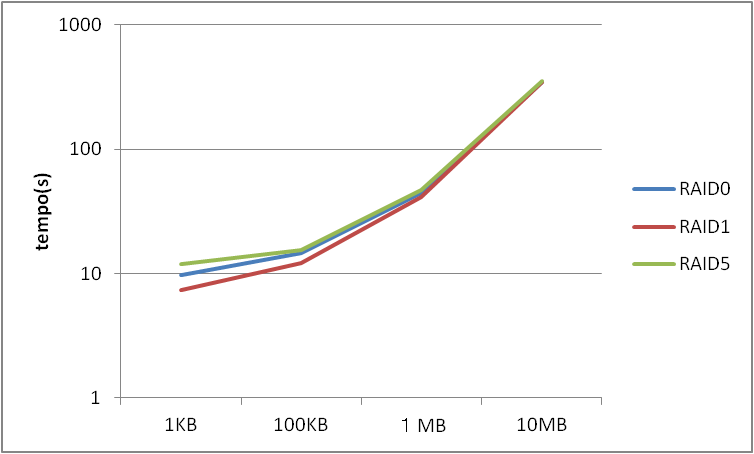
\includegraphics[clip,width=10.0cm]{images/resultados/latencia_leitura.png}
			\caption{Gráfico de leitura para teste de latência}
			\label{fig:lat_leit}
		\end{center}
	\end{figure}
	
	A Figura~\ref{fig:lat_esc} mostra o gráfico de resultado para escrita dos arquivo para cada tipo de RAID.
	
	\begin{figure}[htb]
		\begin{center}
			
			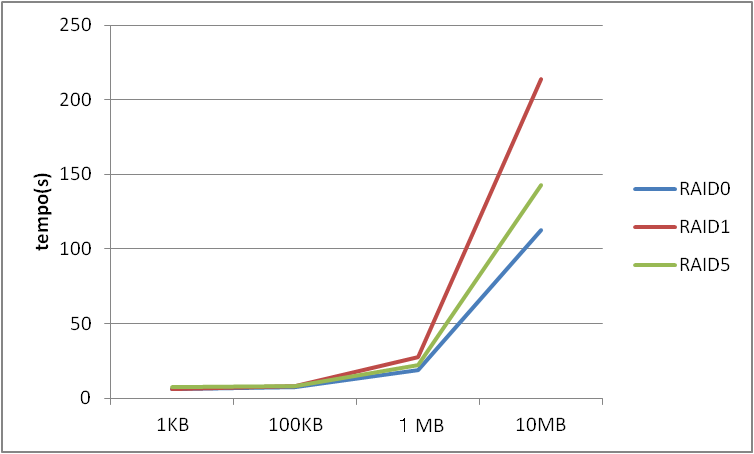
\includegraphics[clip,width=10.0cm]{images/resultados/latencia_escrita.png}
			\caption{Gráfico de escrita para teste de latência}
			\label{fig:lat_esc}
		\end{center}
	\end{figure}
	
	\subsubsection{Teste de vazão}	
	
	\section{Conclusões do Capítulo}

	\section{Resultados}
	Esta sessão apresenta e analisa os resultados obtidos com a realização de testes descritos anteriormente.
	\\
	
	\subsubsection{Teste de latência}
	Primeiramente descreve o resultado do processo de leitura para teste de latência.
	Como no gráfico da Figura~\ref{fig:latencia_l} é difícil distinguir as linhas de cada RAID por ter valores de latência bem próximos entre eles, foi colocado a Tabela~\ref{tab:latencia_l} para mostrar a diferença dos valores.
	Os resultados representam a média dos 1000 operações, descartando-se 10\% dos com maior desvio.
	 \\
	 
	De acordo com Tabela~\ref{tab:latencia_l} o RAID 1 apresenta menor valor de latência entre todos os tipos de RAID quando o arquivo tem tamanho de 1KB ou 100KB. Contudo, quando os arquivos crescem de tamanho, ficando com 1MB e 10MB, o resultado reverte deixando o RAID 1 com a latência mais alta de todos. 
	Isso pode ser explicado pelo fato de que nos RAID 0 e RAID 5 ocorrem a reconstrução de arquivo a partir de alguns pedaços de dados, cujo este procedimento extra possui maior custo de tempo que a transmissão de dados quando trata de arquivos pequenos. Porém, o custo entre dois se aproxima conforme aumenta o tamanho do arquivo e a sua relação inverte quando ultrapassa de um determinado tamanho.
	%Olhando no gráfico da Figura~\ref{fig:latencia_l} esta inversão ocorre aproximadamente no ponto intermediário entre tamanhos de 100KB e 1MB, tanto para RAID 0 quanto para RAID 5, dando um valor aproximado de 500KB.
	\\
	
	Também existe o fato de que no RAID 1 ocorre simples espelhamento de dados, significando que para obter o arquivo basta comunicar com um dos servidores, enquanto nos outros dois tipos de RAID os clientes sempre necessitam se comunicar com múltiplos servidores para realizar a mesma operação. Por isso, o RAID 1 tem possibilidade de concluir a operação de forma mais rápida que RAID 0 e RAID 5. Porém, como a conexão entre cliente e os servidores de armazenamento foi implementado em forma de \textit{multithread}, aparentemente as transmissões que ocorrem entre eles acontecem simultaneamente quando realiza uma operação. Por isso, supormos que a sua influência pode não ser muito grande suficiente a ponto de mudar o resultado do teste.
	\\
	
	Assim, pelos fatos acima apresentados e pelos valores da Tabela~\ref{tab:latencia_l}, é possível considerar que no processo de leitura do arquivo a latência para cada tipo de RAID tem relação de RAID 0 < RAID 5 < RAID 1, sendo como exceção quando trata de arquivos menores.
	\\
	
	\begin{figure}[h]
		\begin{tabular}{lc}
			\begin{minipage}{.50\textwidth}
				\begin{center}
					
					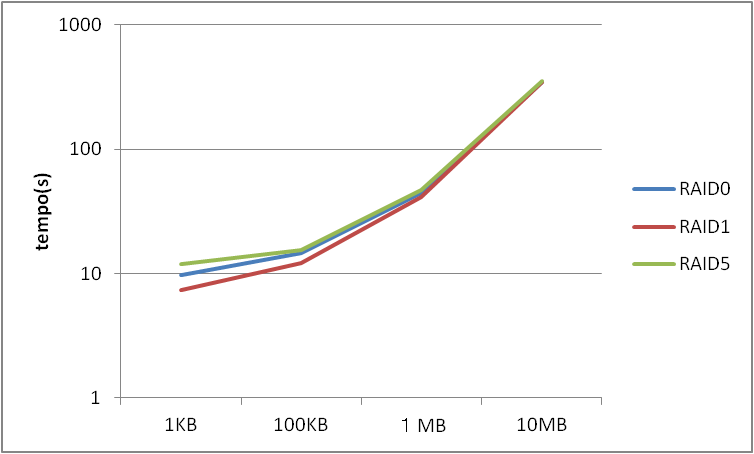
\includegraphics[clip,width=8.0cm]{images/resultados/latencia_leitura.png}
					\caption{Gráfico de latência pata leitura}
					\label{fig:latencia_l}
					
				\end{center}
				
			\end{minipage}
			
			\begin{minipage}{.5\textwidth}
				\makeatletter
				\def\@captype{table}
				\makeatother
				\caption{Tabela de latência pata leitura(s)}
				\label{tab:latencia_l}
				\begin{center}
					\begin{tabular}{|c|c|c|c|c|} \hline
								& 1KB  & 100KB & 1MB   & 10MB  \\ \hline
						RAID 0	& 9.33 & 12.26 & 38.84 & 324.73\\ \hline
						RAID 1	& 9.01 & 12.19 & 41.50 & 348.15\\ \hline
						RAID 5	& 9.76 & 12.62 & 40.11 & 326.75\\ \hline
						
						
					\end{tabular}
				\end{center}
				
			\end{minipage}
		\end{tabular}
	\end{figure}
	
	
	%A Figura~\ref{fig:latencia_e} mostra o gráfico e a Tabela~\ref{tab:latencia_e} mostra a tabela de resultado do teste para escrita de arquivos.
	
	No caso de teste para escrita de arquivo a diferença dos valores da latência para cada tipo de RAID ficou bem nítida comparado com resultado obtido na operação de leitura, como mostram a Figura~\ref{fig:latencia_e} e a Tabela~\ref{tab:latencia_e}.
	\\
	
	De acordo com o gráfico da Figura~\ref{fig:latencia_e}, o crescimento da linha de RAID 1 é mais intensa de todos, onde é esperado que a diferença comparado com outros tipos de RAID tende a aumentar cada vez que o tamanho de arquivo cresce.
	\\
	
	No gráfico aparentemente o RAID 1 possui a maior latência de todos para qualquer tamanho do arquivo. Contudo, olhando na Tabela~\ref{tab:latencia_e} percebe-se que para os arquivos de 1KB e 100KB o RAID 5 apresenta maior latência do que o RAID 1. Isto pode ser explicado com a mesma razão que ocorreu em teste para leitura, onde se o tamanho do arquivo é pequeno o tempo para dividir o arquivo em pedaços de dados é mais demorado que o tempo para enviar estes dados. Aproximadamente a partir de 100KB, a latência do RAID 1 supera o valor dos RAID 0 e RAID 5, de acordo com gráfico. 
	\\
	%Também pode ser citado que no RAID 5 existe uma etapa extra de criar o bloco de paridade e que 
	
	Mesmo para operação de escrita a latência mantém relação de RAID 0 < RAID 5 < RAID 1 para maioria dos casos, ou seja, quando trata de arquivos com tamanhos maiores que 100KB.
	\\
	
	\begin{figure}[h]
		\begin{tabular}{lc}
			\begin{minipage}{.50\textwidth}
				\begin{center}
					
					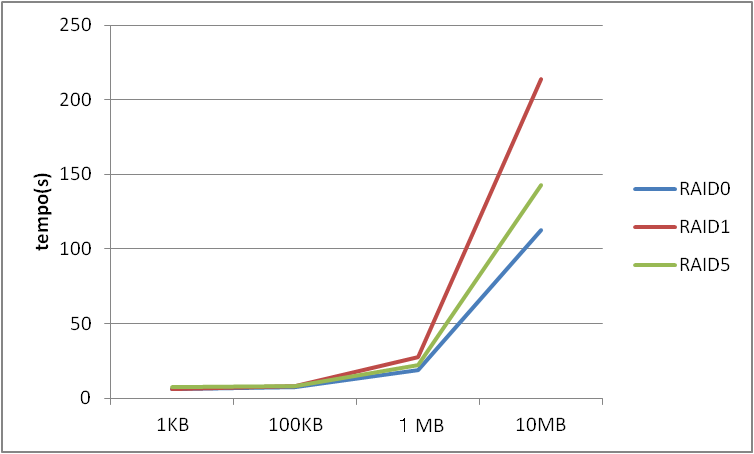
\includegraphics[clip,width=8.0cm]{images/resultados/latencia_escrita.png}
					\caption{Gráfico de latência pata escrita}
					\label{fig:latencia_e}
					
				\end{center}
				
			\end{minipage}
			
			\begin{minipage}{.5\textwidth}
				\makeatletter
				\def\@captype{table}
				\makeatother
				\caption{Tabela de latência pata escrita(s)}
				\label{tab:latencia_e}
				\begin{center}
					\begin{tabular}{|c|c|c|c|c|} \hline
								& 1KB  & 100KB & 1MB   & 10MB \\ \hline
						RAID 0	& 6.70 & 6.91 & 14.92 & 101.93\\ \hline
						RAID 1	& 6.79 & 7.53 & 23.79 & 213.94\\ \hline
						RAID 5	& 7.31 & 7.91 & 18.26 & 134.31\\ \hline
						
					\end{tabular}
					
				\end{center}
			\end{minipage}
		\end{tabular}
	\end{figure}
	
	\subsubsection{Teste de vazão}
	Agora apresentamos a descrição do resultado obtido no teste de vazão, para operação de leitura de arquivo. O gráfico e os valores são mostrados respectivamente nas Figura~\ref{fig:throughput_l} e Tabela~\ref{tab:throughput_l}.
	\\
	
	Neste resultado também o RAID 1 mostrou o comportamento já visto no teste de latência, onde os arquivos de tamanhos de 1KB e de 100KB possuírem maiores valores de vazão de todos, enquanto tamanhos de 1MB e 10MB apresentam menores valores de todos. A explicação para este fato pode ser a mesma que foi analisado no teste anterior, o que considera a relação de custo de tempo entre o processo de reconstrução e a transmissão de dados.
	\\
	
	No gráfico da Figura~\ref{fig:throughput_l} podemos observar que a linha de RAID 0 supera a linha de RAID 1 no ponto aproximado de 250KB, enquanto a linha de  RAID 5 somente consegue superar no ponto aproximado de 500KB. 
	Esta diferença relativamente grande de tamanho para superar a linha do RAID 1 não foi observado no teste de latência, apresentando tamanhos bem próximos entre RAID 0 e RAID 5. Este fato pode ser explicado por existência de vários clientes em operação ao mesmo tempo, diferentemente do teste de latência que existia um único cliente, cujo a pequena diferença do custo de tempo entre RAID 0 e RAID 5 não foi explícita.
	\\
	
	Depois que o tamanho do arquivo passa de 1MB, as linhas da taxa de vazão dos três tipos de RAID começam a se aproximar, aparentemente convergindo em um único valor no ponto de 10MB. Porém, pela Tabela~\ref{tab:throughput_l} é possível observar que a relação das taxas ainda continuam RAID 0 < RAID 5 < RAID 1.
	\\
	
	Em geral, exceto quando trata de arquivos maiores que 500KB, podemos considerar que a taxa de vazão para leitura de arquivo entre três tipos de RAID obedecem a relação de RAID 0 > RAID 5 > RAID 1, como esperado.
	\\
	
	\begin{figure}[h]
		\begin{tabular}{lc}
			\begin{minipage}{.50\textwidth}
				\begin{center}
					
					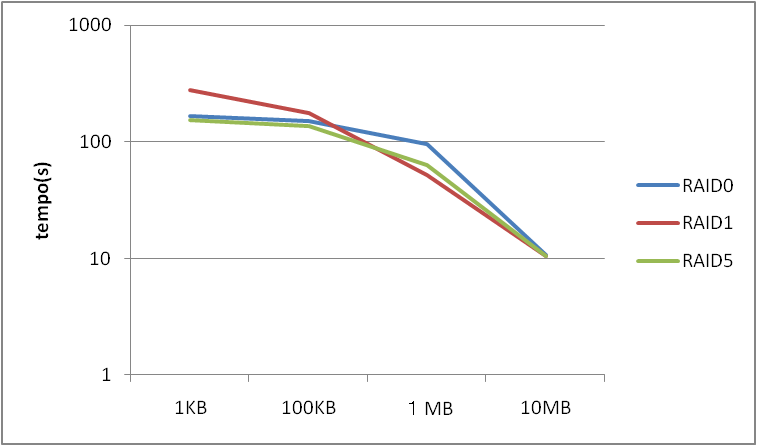
\includegraphics[clip,width=8.0cm]{images/resultados/throughput_leitura.png}
					\caption{Gráfico de vazão para leitura(ops/s)}
					\label{fig:throughput_l}
					
				\end{center}
				
			\end{minipage}
			
			\begin{minipage}{.5\textwidth}
				\makeatletter
				\def\@captype{table}
				\makeatother
				\caption{Tabela de vazão para leitura(ops/s)}
				\label{tab:throughput_l}
				\begin{center}
					\begin{tabular}{|c|c|c|c|c|} \hline
						& 1KB & 100KB & 1MB & 10MB \\ \hline
						
						RAID 0	& 167.14 & 151.63 & 95.08 & 10.63\\ \hline
						RAID 1	& 278.86 & 177.43 & 51.92 & 10.52\\ \hline
						RAID 5	& 152.79 & 135.30 & 63.34 & 10.56\\ \hline
						
					\end{tabular}
				\end{center}
				
			\end{minipage}
		\end{tabular}
	\end{figure}
	
	
	O último experimento feito é o teste de vazão para escrita de arquivos.
	Diferentemente dos resultados obtidos pelos testes anteriores, em que o RAID 1 apresentava melhor desempenho para casos de arquivos pequenos, o gráfico da Figura~\ref{fig:throughput_e} mostra que o RAID 0 apresenta o melhor valor para a taxa de vazão independentemente de tamanho do arquivo. 
	Contudo, observando a inclinação das linhas de RAID 0 e RAID 1, supomos que a inversão do custo de tempo entre a divisão de arquivo e o envio de dado já acontecem em algum tamanho menor que 1KB. Assim, podemos considerar que este gráfico também apresenta o mesmo comportamento visto nos testes anteriores. 
	\\
	Em tamanho aproximado de 25KB a linha de RAID 5 ultrapassa a linha de RAID 1 e depois que o tamanho do arquivo chega em 100KB, todas as linhas de RAID começam a prosseguir de forma quase paralela entre si.
	\\
	
	Assim, quando consideramos arquivo de tamanhos maiores que 25KB, a taxa de vazão entre os três tipos de RAID possui relação de RAID 0 > RAID 5 > RAID 1.
	\\
	
	\begin{figure}[h]
		\begin{tabular}{lc}
			\begin{minipage}{.50\textwidth}
				\begin{center}
					
					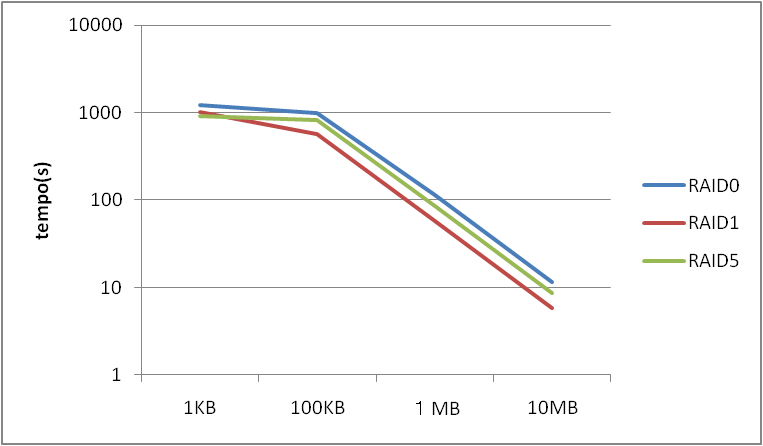
\includegraphics[clip,width=8.0cm]{images/resultados/throughput_escrita.png}
					\caption{Gráfico de vazão para escrita}
					\label{fig:throughput_e}
					
				\end{center}
				
			\end{minipage}
			
			\begin{minipage}{.5\textwidth}
				\makeatletter
				\def\@captype{table}
				\makeatother
				\caption{Tabela de vazão para escrita(ops/s)}
				\label{tab:throughput_e}
				\begin{center}
					\begin{tabular}{|c|c|c|c|c|} \hline
						& 1KB & 100KB & 1MB & 10MB \\ \hline
						
						RAID 0	& 1209.19 & 988.14 & 113.07 & 11.51\\ \hline
						RAID 1	& 1023.54 & 571.43 & 58.01  & 5.76 \\ \hline
						RAID 5	& 914.91  & 830.56 & 84.52  & 8.66 \\ \hline
						
						
					\end{tabular}
				\end{center}
				
			\end{minipage}
		\end{tabular}
	\end{figure}
	
	\section{Conclusões do Capítulo}
	
	Depois de obter os resultados dos testes, foi possível verificar que o desempenho para leitura e escrita de dados entre os três tipos de RAID possui a relação de RAID 0 > RAID 5 > RAID 1 na maioria dos casos. Observando que 500KB foi o maior tamanho aproximado em que ocorre a inversão da relação de custo de tempo entre a transmissão de dados e o processo de divisão ou reconstrução de arquivo, quando trata de arquivos com tamanho desta ordem a vantagem que RAID 1 tem sobre RAID 5 pode ser considerado bem pequena. 
	Por exemplo, na latência para leitura de arquivo de 100KB o RAID 1 ganha do RAID 5 somente por 0,43 segundos, enquanto para arquivo de 1MB o RAID 5 é 1,39 segundos mais vantajoso que o RAID 1.
	\\
	
	Assim, podemos dizer que o RAID 5 conseguiu cobrir as desvantagens que existem nos RAID 0 e RAID 1, conseguindo ter a segurança nos arquivos armazenados sem perder muito o desempenho para a transmissão e o armazenamento.
	\\
	
	
	
	
	
	
	
	
	
	
	
	
	
\chapter{Conclusões e Trabalhos Futuros}
Neste capítulo iremos apresentar as conclusões obtidas com os resultados dos experimentos realizados, além de uma breve explanação sobre quais são os rumos que podem ser tomados a fim de evoluir o sistema, quais melhorias podem ser realizadas de modo a garantir um programa mais robusto e confiável.
\\

\section{Conclusões}
%Após a construção do sistema e a análise realizada sobre os dados coletados em nossos experimentos foi possível levantar algumas conclusões sobre o nosso sistema de arquivos distribuídos baseado nos conceitos de RAID.


Neste trabalho conseguimos construir um sistema de arquivos distribuídos tolerante a falha, cujo o sistema consegue assegurar a confiabilidade dos arquivos armazenados usando os conceitos de RAID e o serviço fornecido pelo sistema é protegido através de uso da biblioteca \textit{BFT-SMaRt}.
Os resultados obtidos no experimento confirmam que realmente o RAID 5, que usa abordagem de geração paridade, tem melhor eficiência para transferência de dados comparado ao RAID 1, que usa a replicação de arquivo, perdendo apenas para RAID 0, que focaliza em ter maior desempenho sem preocupar na segurança dos arquivos.
Assim, conseguimos mostrar as vantagens de adotar os concentos de RAID na construção do sistema de arquivos distribuídos, na parte de conjunto de armazenamento de dados. Acreditamos que o RAID 5 seria uma opção adequada para casos que necessitam satisfazer condições de desempenho razoável para operações dos arquivos, possibilitando manter a segurança dos dados armazenados com custo de espaço relativamente menor.
\\


\section{Trabalhos Futuros}

Neste trabalho foi realizado os experimentos com objetivo de fazer a comparação de desempenho para armazenamento de arquivos entre três tipos de RAID, dando mais ênfase em operação de leitura e escrita de dados.
Mas ainda podem ser feitos outros tipos de experimentos para fazer as comparações, como verificar o que acontece com relação ao desempenho dos tipos de RAID quando aumenta o número de servidores em operação ou comparar a eficiência de recuperação de um arquivo entre RAID 1 e RAID 5. Também pode-se estender o sistema para suportar outros tipos de RAID, além de testá-los em casos de falhas.
\\

Atualmente todo o gerenciamento realizado pelo serviço de metadados ocorre em tempo de execução, sendo salvo apenas em memória, pretendemos modificar o código para que o mesmo possibilite que as informações gerencias sejam armazenadas em disco, memória não volátil. Pois da forma realizada atualmente, toda vez que o sistema é iniciado as informações gerencias estão em branco, ou seja, todos os blocos de arquivos armazenados no serviço de armazenamento não passam de lixo, espaço de disco desperdiçado. Quando o serviço de metadados estiver integrado com algum tipo de banco de dados esses dados serão preservados mesmo quando os servidores precisarem ser desligados por qualquer motivo.
\\

Visto os resultados obtidos em nossos experimentos, observamos que o sistema comporta, sem diminuir drasticamente o tempo de resposta, cinquenta usuários simultâneos  solicitando diversas operações, pretendemos estudar modos para aumentar essa quantidade, de modo que o nosso sistema possa ser usado em um ambiente real.
Além disso, na realização de experimentos foi observada a ocorrência de algumas exceções durante a execução do programa nas máquinas remotas de servidores de armazenamento. As exceções foram de \textit{OutOfMemoryError: Java heap space}, causado pela possível falta de memória disponível no JVM, a máquina virtual de java, e de \textit{OutOfMemoryError: GC Overhead limit exceeded}, a exceção que ocorre quando o coletor de lixo de java consome a maioria de tempo de execução desalocando componentes desnecessários da memória, impedindo que o programa prossegue a sua tarefa.
Durante experimento elas foram evitadas mudando a configuração básica do JVM, aumentando a capacidade máxima da memória que pode utilizar. Contudo, como não podemos considerar que todos os computadores são equipados com memória suficiente para executar o nosso sistema, é necessário que seja feito a redução de uso da memória por sistema. 
Como neste trabalho foi focalizado principalmente em construção do sistema, o código fonte do programa ainda pode ser revisado e otimizado, assim, conseguindo o melhoramento em relação ao uso da memória e, se for possível, o aumento no desempenho do sistema todo.
\\




\postextual

\bibliographystyle{plain}

\bibliography{bibliografia}


\end{document}


